% This is LLNCS.DEM the demonstration file of
% the LaTeX macro package from Springer-Verlag
% for Lecture Notes in Computer Science,
% version 2.4 for LaTeX2e as of 16. April 2010
%
\documentclass{llncs}
%
\usepackage{amsmath}
\usepackage{amssymb}
\usepackage{algorithm}
\usepackage{algorithmic}
\usepackage{graphicx}
\usepackage{subfigure}
\usepackage{makeidx}  % allows for indexgeneration

% new command for algorithmic input and output
\renewcommand{\algorithmicrequire}{\textbf{input:}}
\renewcommand{\algorithmicensure}{\textbf{output:}}

%
\begin{document}
%
\frontmatter          % for the preliminaries
%
\pagestyle{headings}  % switches on printing of running heads
%

%% \tableofcontents
%% \mainmatter

%% \chapter*{Preface}
%

this is preface

\vspace{1cm}

\begin{flushright}\noindent
Nov 2017\hfill Walter Olthoff\\
Program Chair\\
NASAC'17
\end{flushright}

% !TEX root = ../paper.tex
% header
%

\title{Parallel Evolutionary Algorithm in Solving Single Objective Software Project Management Problem\vspace{-1em}}
%Solving Project Management Problem with Parallel Evolutionary Algorithm}
%
\titlerunning{Project Management}  % abbreviated title (for running head)
%                                     also used for the TOC unless
%                                     \toctitle is used
%
\author{ Jinghui Hu \and Xu Wang \and Jian Ren \and Chao Liu}
%
\authorrunning{Hu, Wang, Ren, Liu} % abbreviated author list (for running head)
%
%%%% list of authors for the TOC (use if author list has to be modified)
\tocauthor{Jinghui Hu, Xu Wang, Jian Ren, Chao Liu}
%
\institute{\vspace{-1em}
State Key Laboratory of Software Development Environment,\\
School of Computer Science and Engineering, 
\\Beihang University, Beijing 100191, China
%\\
%\email{\{hujinghui, bhwangxu, renjian, liuchao\}@buaa.edu.cn}
%\thanks{supported by the Chinese National Natural Science Foundation (6160050441)}
}



\maketitle

\begin{abstract}
\vspace{-0.8cm}
Software project management problem mainly includes resources allocation and work packages scheduling.
This paper presents an approach to Search Based Software Project Management based on paralleled implementation of evolutionary algorithm on GPU. 
Our approach aims to paralleled the genetic operators including: crossover, mutation and evaluation in the evolution process to achieve faster execution time for the optimization process.
To evaluate our approach, we conducted a ``proof of concept'' empirical study, using data from three real-world software projects. 
Both sequential and parallel version of a conventional single objective evolutionary algorithm are implemented. 
%The objective is to minimize the overall duration a software project, while satisfying the dependencies between work packages and constraints of resources allocation in the software project.
The sequential version application is based on common programming approach using C++ programming language, and the parallel version application is based on GPGPU programming approach using CUDA C++ API.
We redesign search based evolutionary algorithm to cater for our purpose of parallel programming on GPU.
Results indicate that even a relatively cheap graphic card (GeForce GTX 970) can speed up the optimization process significantly.
We believe that deploy parallel evolutionary algorithm based on GPU  may fit many applications for other software project management problems, since software projects often have complex inter-related tasks and resource and are typically characterized by large scale problems that need to be paralleled to improve execution time.


\keywords{Software project management, Evolutionary algorithm, Parallel Optimization Problem}
\end{abstract}

% !TEX root = ../paper.tex
%% chapter 1
\section{Introduction}
\vspace{-2mm}
%\subsection{Background}
%
%In our daily life, each of us are facing many tasks. How to properly arrange those tasks is an emerging research topic in academia. 
In an actual
development process of software project, the project manager's responsibility is
to properly schedule the tasks of software project development, supervise the
programming work of the software engineer and arrange the whole development
progress of the software to ensure that the software can be delivered before the
deadline~\cite{stellman}. 
Therefore, the project management problem is not only
a very fundamental problem in software engineering, but also a very difficult
problem in the actual work for the project manager.

In fact, software project management is an art of staff management and task scheduling in software engineering. It requires an overall understanding of the lifecycle of software development, such as planning tasks, staff organization and so on. 
Through a survey on the practice of software project management~\cite{chang,alba,ren,penta}, we found that the different task management designed by the project manager, such as  the arrangement order of the work packages in a project, or the different  resource allocation in the same human resources team, will have a great  impact on the project's overall duration.
Excellent project managers can  shorten the overall duration by arranging the order of tasks, making full use  of the team's resources or allocating human resources properly. However, at the beginning of a software project, the project managers need to spend a lot  of time on the discussion that what kind of difficulties will be faced in the process of development and the detail of resources allocation in  software engineering phase~\cite{pentico}, such as requirements analysis, system design, system development, system testing etc. 

However, an automatic method to properly arrange the entire software project management process is still lacking. 
We target at two typical difficulties preventing automatic techniques to be realized into a real world project: 
1) the complexity of the problem model causes difficulties when a project manager is formalizing the problem he\slash she is facing, 
2) the execution time of the optimization process is quite often unbearable comparing to the result it yields. 

In this paper, we introduce a framework to deploy a conventional evolutionary algorithm to solve the work package scheduling problem as a single objective optimization problem. 
And by catering the most computation intensive portion of algorithm to run on a parallel manner, this framework speeds up the execution of optimization process significantly.
With an empirical study on three real world software project data, we show how this framework can ease above mentioned two typical problems that most of the existing optimization techniques to project management are facing.
We claim that heuristics provides mangers with intuitive features towards ``simple-to-deploy'', and parallel computation running on GPU provides faster execution time.

The main purpose of this paper is to push forward the automated software project management powered by the search-based approach, which is an important component of search-based software engineering (SBSE) and also a future development trend of software engineering project management in the era of big data and parallel computing.

The rest of this paper is organized as follows. First, we give a brief background of evolutionary algorithm and software project management problem in Section 2 and 3. Then we introduce the design of algorithm implemented in a parallel manner in Section 4. Section 5 presents the results of empirical study. In Section 6, we provide a brief overview of related work before concluding in Section 7.







% !TEX root = ../paper.tex

\section{Evolutionary Algorithm}

\subsection{Meta-heuristic Algorithms}
%
In the development process of computer science, the design of program 
algorithm provides much power to promote the advancement of computer science 
and technology. We know that in solving the similar kind of problem, the 
computational efficiency of different algorithms is completely different. 


Algorithm has become the soul to solve practical problems using computer. In
addition to the classical algorithm that can be used to calculate a certain
problem at a given time, a class of algorithms is found with different
performance. The nature of this algorithm is that no performance guaranteed can
be given in theory but is often possible to give the solution of the problem
efficiently in practice. This class of algorithms is called meta-heuristic
algorithm.

Unlike the traditional algorithm, the meta-heuristic algorithm tries to 
provide one or more disaggregation in one calculation, and the corresponding 
optimal solution can be found in the process of searching. The meta-heuristic 
algorithm can often find a good solution, but there is no way to prove that 
it will not get a worse solution, or cannot even find solution. The 
evolutionary algorithm used in this paper usually gives an approximate 
optimal solution within a given time, but can not to ensure that this solution 
is best at a given time.

In reality, there are some extreme situations in the process of implementing 
the heuristic algorithm, that is, some solutions that the meta-heuristic 
algorithms need are difficult to find or they cannot be found at all. The 
heuristic algorithm is often used to solve some Non-Deterministic Polynomial 
complete problems(NPC) because the calculative requirement of NPC is very 
large so some deterministic algorithms cannot be used to find the optimal 
solution. However, the meta-heuristic algorithm can get a good answer in a 
reasonable time when dealing with NPC, so the meta-heuristic algorithm is 
also a hot field for academic community.

The thought of the meta-heuristic algorithm has been formed for a long time 
and since its formation, the research on it has not been interrupted. As a 
result, there are many ways to achieve it. In recent decades, the research of 
meta-heuristic algorithm has developed rapidly, and there have been many more 
mature and specific subalgorithms. In the 1970s, Professor Holland~\cite{holland} 
proposed genetic algorithm. Genetic algorithm simulates the 
evolutionary method of biological population to find the optimal solution of 
some problems, which opens up a new upsurge in research on meta-heuristic 
algorithm. Ever since the 1980s, a number of new meta-heuristic algorithms emerged~\cite{harman}, 
such as Simulated Annealing Algorithm, Artificial Neural Network, Tabu Search 
and etc.. 
%What are concerned greatly among them are  Evolutionary Algorithm, Ant Algorithms, Genetic Quantum Algorithm, etc..

% text moved to previous section



\subsection{Evolutionary algorithm}

Evolutionary algorithm~\cite{deb} origins from Darwin's theory of evolution and Mendel's 
theory of genetic gene. Its essence is an efficient global search algorithm 
that imitates the biological evolution of nature. In the process of searching 
for the optimal solution, it can automatically acquire and accumulate the 
more optimal individual in the large population, and control search process 
adaptively. It can converge to the better solution oriented according to the 
natural law of the strong stronger and the weak weaker.


The core of the evolutionary algorithm is the design of encoding of candidate
solutions and the fitness function. The evolutionary algorithm first encodes the
solutions according to the different requirements of problem. each individual in
the population represents a solution to the problem. At the same time, for each
solution of the problem, we also need to design the fitness function. The
fitness value of different solutions is used to measure the adaptability of
different individuals. Individuals with high adaptability are more likely to
survive in the evolution process of population. After encoding, there are four
steps including initialized population, crossover, mutation and selection. The
specific operation of initialized population is to generate the first generation
of population randomly; The cross is to product new offspring population by the
individual hybridization between parents then the mutation is to mutate certain
genes in the individuals and mutated individuals will be involved in population
hybridization to maintain the species diversity of the population. As a result,
the operation above will bring some novel solutions; Finally, the selection is
to choose better individuals in the whole population according to the natural
law of winning.  In a word, the evolutionary algorithm obtains the optimal
solution by the evolution of the population.




% !TEX root = ../paper.tex
% chapter3

\section{Project Management Problem}
%

\subsection{Project Plan}
%

The core of project management problem is work package scheduling and resource
allocation.
Figure \ref{fig:sample} is a Gantt chart of typical software project management, which
illustrates work package arrangement of a real industry software engineering.
Generally, all the important phases in software engineering, such as project
planning, requirements analysis, design, development, testing, deployment etc., are inseparable from the allocation of work packages.  These work
packages have a mutually restrictive relationship. Some work packages must be
started when other work packages are completed. For instance, the analysis of
software requirements is often to take place after the completion of project planning
while some work packages can be done at the same time, and there is no
impact on each other, such as software development and software testing can
often be synchronized. The goal of project manager is using the shortest possible time
to complete all work packages within the software project duration.

% figure 2
%\vspace{-6mm}
\begin{figure}[!ht]
  \centering
%  \vspace{-6mm}
  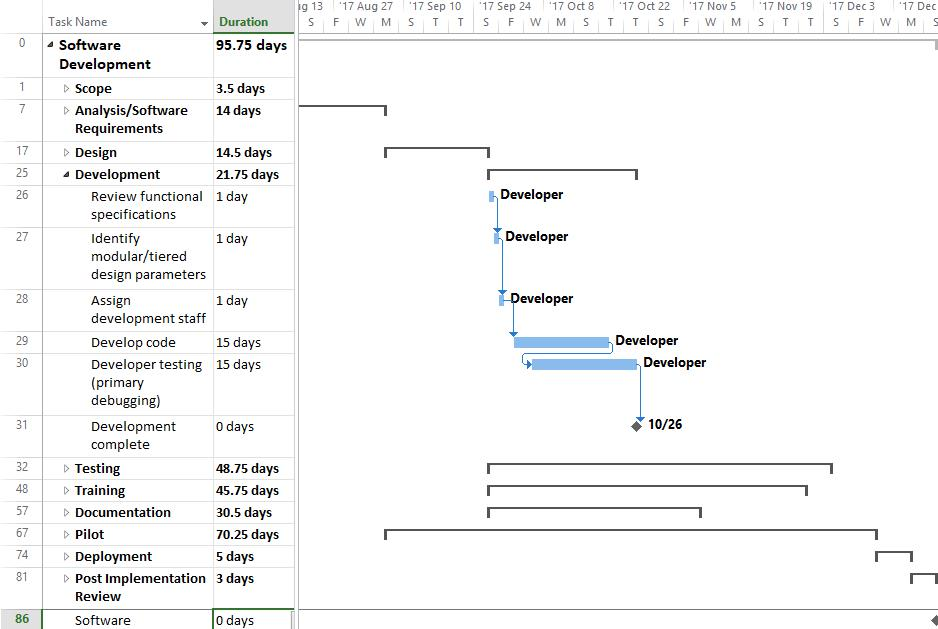
\includegraphics[width=0.9\textwidth]{figures/pm_sample.jpg}
  \vspace{-2mm}
  \caption{Software Project Plan in a Microsoft Project File (.mpp)}
  \label{fig:sample}
  \vspace{-2mm}
\end{figure}


\begin{figure}[!ht]
  \centering
  \vspace{-3mm}
  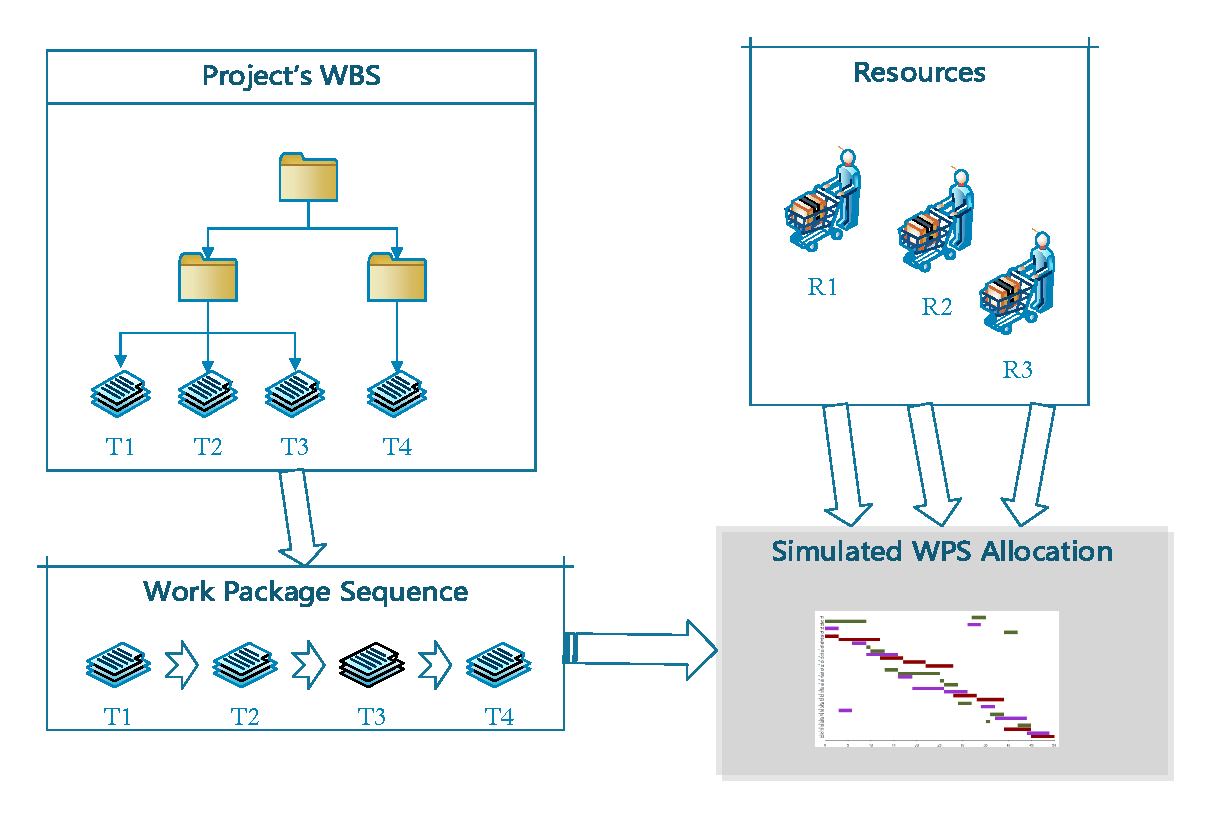
\includegraphics[width=0.8\textwidth]{figures/simu.pdf}
  \vspace{-5mm}
  \caption{Project Plan of Software Development}
  \label{fig:simu}
\vspace{-5mm}
\end{figure}


 In the process of project management, the work packages in the project are
 allocated by simulation. See figure \ref{fig:simu}, Firstly, the whole project
 is decomposed into several work packages by \emph{work breakdown structure},
 and those work packages are arranged into a corresponding \emph{work package
   sequence}. Secondly, according to the dependencies of the work packages and
 the restriction of resource, each kinds of resources is allocated to the
 corresponding work package by \emph{first-come-first-served}
 algorithm. Finally, the project's overall duration is yielded from the simulation.



\subsection{Definition and Assumptions}
%
The goal of this paper is to find an optimal solution or near optimal
solution for the project management problem described as follows:


\emph{
  For a software project with $N$ work packages and $M$ kinds of resources,
  there is a corresponding dependency between these work packages, and each
  resource can only be assigned to the specified work package.  It is necessary
  to arrange the order of the work package reasonably and make the overall
  construction duration as short as possible under the condition of satisfying
  the work package dependency and the resource allocation restriction.
}

%
There are three assumptions for our project management problem.

Assumption I: The software project plan can be decomposed into a set of
work packages containing $N$ elements $T = \{t_1, t_2, ..., t_N \}$.
Each work package in set $T$ is indivisible (i.e., The work package cannot be
split to other work package in the schedule), the set of work packages have a
pre-estimated workload, the composition of the workload is the collection
$E = \{e _1, e_2, ..., e_N \}$. The function $TE: T \rightarrow E$,
the mean of this function is that for a given work package $t_i$, produces an
estimated workload $e_i = TE(t_i)$ for a work package $t_i$, where $e_i$ is the
estimated workload of $t_i$.


Assumption II: The work packages in the software project  can be
processed with $M$ kinds of resources, which constitute a resource set
$R = \{r_1, r_2, ..., r_M \}$, for each project's work package set $T$ and the
resource set $R$, There exists a function $TR: T \times R \rightarrow \{0, 1\}$,
for the given work package $t_i$ and the resource $r_j$, $TR(t_i, t_j) = 1$
means the resource $r_j$ can be allocated to the work package $t_i$, while
$TR(t_i, r_j) = 0$ means cannot.


Assumption III: All work packages in the set $T$ of the software project
plan have dependencies. These dependencies form a set
$Dep= \{t_i \rightarrow t_j \mid t_i, t_j \in T, t_j \text{ depends on } t_i\}$.
As the assumption of this paper, $t_i \rightarrow t_j$ means that $t_j$ depends
on $t_i$, that is the work package $t_j$ must be arranged after the work
package $t_i$, and satisfy the formula $t_j.start \leq t_i.end$ (where $t.start$
and $t.end$ respectively indicate the start time and the end time of the work
package $t$).  And assume that there is no direct or indirect "loop" dependency
between work packages.


  \vspace{-2mm}


\subsection{The Objective of Problem}
%
The objective of project management is to find an optimal work package sequence
under the three assumptions above.
The notation of work package sequence(WPS) is as follows:
\begin{equation}
\vspace{-2mm}
  S = \{
  (t_{p_1}, r_{q_1}) ... \rightarrow (t_{p_j}, r_{q_j}) \rightarrow ... (t_{p_N}, r_{q_N})
  \mid t_{p_i} \in T, r_{q_j} \in R
  \}
  \label{wps}
\end{equation}
where every $(t_p, r_q)$ means resource $r_q$ is allocated to work package $t_p$.
The WPS needs to meet the following two restrictions:
\begin{enumerate}
\item $\nexists i < j, t_j \rightarrow t_i \in Dep$.
  (The WPS must satisfy the dependencies)
\item $\nexists i, k, TR(t_i, r_k) = 0$.
  (All work packages must have at least one resource)
\end{enumerate}
For the work package arrangement sequence S, each work package $t$ is given
$t.start$ (the start time) and $t.end$ (the end time).  The total cost duration
function of the project is defined as $f(S) = max\{t.end \mid t \in T\}$. That
is, the overall duration represents the maximum value of the end time of all
work packages in a work package arrangement sequence $S$, which also means when the
last work package of the project is completed, the entire project ends.
The objective function is defined as following:
\begin{equation}
  \text{\textbf{Objective:}    } min(f(S)) = min(max\{t.end \mid t \in T\})
\end{equation}
The objective of the project management problem is to find a work
package sequence $S$ to arrange the whole project under the condition
of satisfying the restriction of dependencies and resources, so that
the overall  duration is minimized.








% !TEX root = ../paper.tex
%
% ---------- chapter 4 ----------
%

\section{Design of Algorithm}
%
This section introduces the two important steps in using the evolutionary
algorithm. One is to choose the representation of the problem's solution, the
other is to define a appropriate fitness function.

%% \begin{figure}[!ht]
%%   \centering
%%   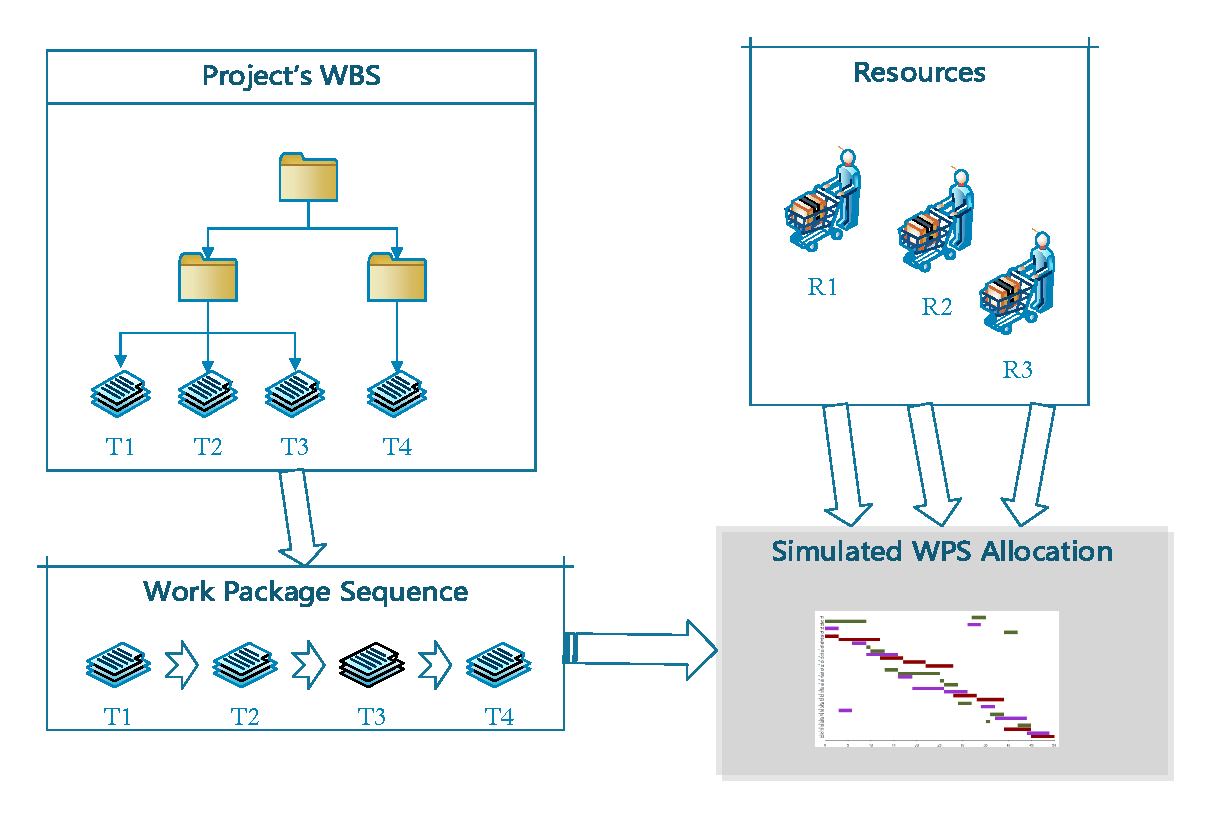
\includegraphics[width=0.8\textwidth]{figures/simu.pdf}
%%   \caption{Project Plan of Software Development}
%%   \label{fig:simu}
%% \end{figure}

%% There are two important steps in using the evolutionary algorithm. One is to
%% choose the representation of the problem's solution, the other is to define a
%% appropriate fitness function. In the process of project management, the work
%% packages in the project are allocated by simulation. See figure \ref{fig:simu},
%% Firstly, the whole project is decomposed into several work packages by
%% \emph{work breakdown structure}, and those work packages are arranged into a
%% corresponding \emph{work package sequence}. Secondly, according to the
%% dependencies of the work packages and the restriction of resource, each kinds of
%% resources is allocated to the corresponding work package by
%% \emph{first-come-first-served} algorithm. Finally, the project's overall
%% duration is calculate by simulation.

  \vspace{-2mm}
\subsection{The Representation of Solution}
  \vspace{-2mm}%
For the above-mentioned problem, the representation of solution is defined as
follows.
This paper uses \emph{work package sequence} (hereinafter referred to as \emph{WPS}) to
represent a solution of project management problem. The representation of such a
solution is actually a priority arrangement sequence of the work packages in
the whole project, and the number of solutions for a project containing the $N$
work packages is $N!$, which is large enough to do random search.
%This is a figure 7
\begin{equation}
  T_1 \rightarrow T_5 \rightarrow T_6 \rightarrow T_4 \rightarrow T_8
  \rightarrow T_3 \rightarrow T_9 \rightarrow T_2 \rightarrow T_7
  \label{repr}
\end{equation}
For example, equation (\ref{repr}) is solution, the solution represents the work
package sequence in the priority of $T_1$, $T_5$, $T_6$, $T_4$, $T_8$, $T_3$,
$T_9$, $T_2$, $T_7$, while arranging the work packages. This representation is
beneficial and intuitive to programming.

  \vspace{-2mm}
\subsection{Fitness Evaluation}
 \vspace{-2mm}
The above-mentioned representation of solution make each individual encoded as
\emph{WPS}. The fitness value of \emph{WPS} is the project's overall duration,
which is calculated by simulating the assignment of work packages in the set of
package sequence, see equation (\ref{wps}).

The Algorithm~\ref{alg} illustrates  how to calculate corresponding project overall
duration. Firstly, according to first-come-first-served
rule, the front work packages in a \emph{WPS} have high priority to get
resources, the back work packages has low priority. Secondly, the $TR$ function
defines which work package can get which resources, if two work packages that
require the same resources, the higher priority one will use the resources
firstly, the lower priority one will use the resources after the higher one
releases the resources. Finally, the project's overall duration is the last end
time after all work packages are allocated the resources.
As we can see from the Algorithm~\ref{alg}, to calculate the overall duration,
the algorithm must traverse all $N$ work packages and $M$ kinds of resources,
so the average complexity of fitness evolution is $O(N \times M)$.

\begin{algorithm}[!h]
  \caption{Fitness Evaluation Algorithm}
  \label{alg}
  \begin{algorithmic}
    \REQUIRE $WPS, R, TE, TR$
    \ENSURE $duration$
    \FOR {$i$ \textbf{from} $1$ \textbf{to} $WPS.length$}
      \STATE $t \gets WPS[i]$
      \STATE $ effort \gets TE(i)$
      \FOR {$r$ \textbf{in} $R$}
        \STATE $r.occupy \gets 0$
      \ENDFOR 
      \FOR {$r$ \textbf{in} $R$}
        \IF{$TR(t,r) = true$}
          \STATE $t.start \gets r.occupy$
          \STATE $t.end \gets r.occupy + effort$
          \STATE $r.occupy \gets t.end$
          \STATE \textbf{break}
        \ENDIF
      \ENDFOR
    \ENDFOR
    \STATE $duration \gets 0$  
    \FOR {$t$ \textbf{in} $WPS$}
      \IF{$t.end > duration$}
        \STATE $duration \gets t.end$
      \ENDIF
    \ENDFOR
  \end{algorithmic}
\end{algorithm}
%\vspace{-10mm}
  \vspace{-2mm}
\subsection{Genetic Operators}
%

There are two main types of operators in evolutionary algorithms:
\emph{crossover} and \emph{mutation}.
\textbf{Crossover}
In evolutionary algorithms, crossover is a genetic operator used to vary the
programming of a chromosome or chromosomes from one generation to the next.  In
this paper, we use a two-point crossover, that is, two points are selected
randomly on the parent organism strings. Everything between the two points is
swapped between the parent organisms, rendering two child organisms then
exchange corresponding part of chromosomes to get offspring individual.
\textbf{Mutation}
In evolutionary algorithms, Mutation is a genetic operator used to maintain
genetic diversity from one generation of a population of genetic algorithm
chromosomes to the next.  In this paper, we use two-point exchange mutation,
that is, two points is selected randomly on individual organisms strings, and
then exchange the two points.

  \vspace{-6mm}
\subsection{Parallel Evolutionary Algorithm}
%
Figure \ref{fig:flow} summarizes the basic process of the evolutionary
algorithm.
Figure \ref{fig:flow:s} is common sequential evolutionary algorithm, the
algorithm has several steps, such as initialization, crossover, mutation, and
selection. Candidate solutions to the optimization problem play the role of
individuals in a population, and the fitness function determines the convergence
of the solutions. Evolution of the population then takes place after the
repeated application of the above operators.
Figure \ref{fig:flow:p} illustrates a parallel evolutionary algorithm. The
parallel one follows most steps in sequential one, but put the top
time-consuming work on GPU. The steps of crossover, mutation and evolution runs
in different cores in GPU so that the speed of calculation can be improved a lot.

  \vspace{-2mm}
\subsection{Runtime Environment}
%
%Both sequential and parallel's application is implemented on Window 7 operating system.

The hardware environment of algorithm implementation is as follows: the runtime
processor that executes the sequential evolutionary algorithm is the Intel i7
series CPU (abbreviated as CPU). The runtime processor of the parallel
evolutionary algorithm is the NVidia GeForce GTX 970 (abbreviated as GPU). The
major difference between CPU and GPU is that they have different number of
computation cores. Normally, the computation speed of a GPU core is lower than a
CPU core. But GPU has far more than the number of CPU cores. In this paper, The
CPU we used has 8 cores and the GPU has 1664 cores.

The software environment that runs application is as follows: the sequential
programs runs on Microsoft Visual Studio 2012 C++ Compiler environment, the
parallel one runs on CUDA 7.0.28 Runtime environment. Both sequential and
parallel application is evaluated in the same computer.

\vspace{-6mm}
\begin{figure}[!ht]
  \centering
  % fisrt figure
  \begin{minipage}{0.29\textwidth}
    \centering
    \subfigure[Sequential] {
      \label{fig:flow:s}
      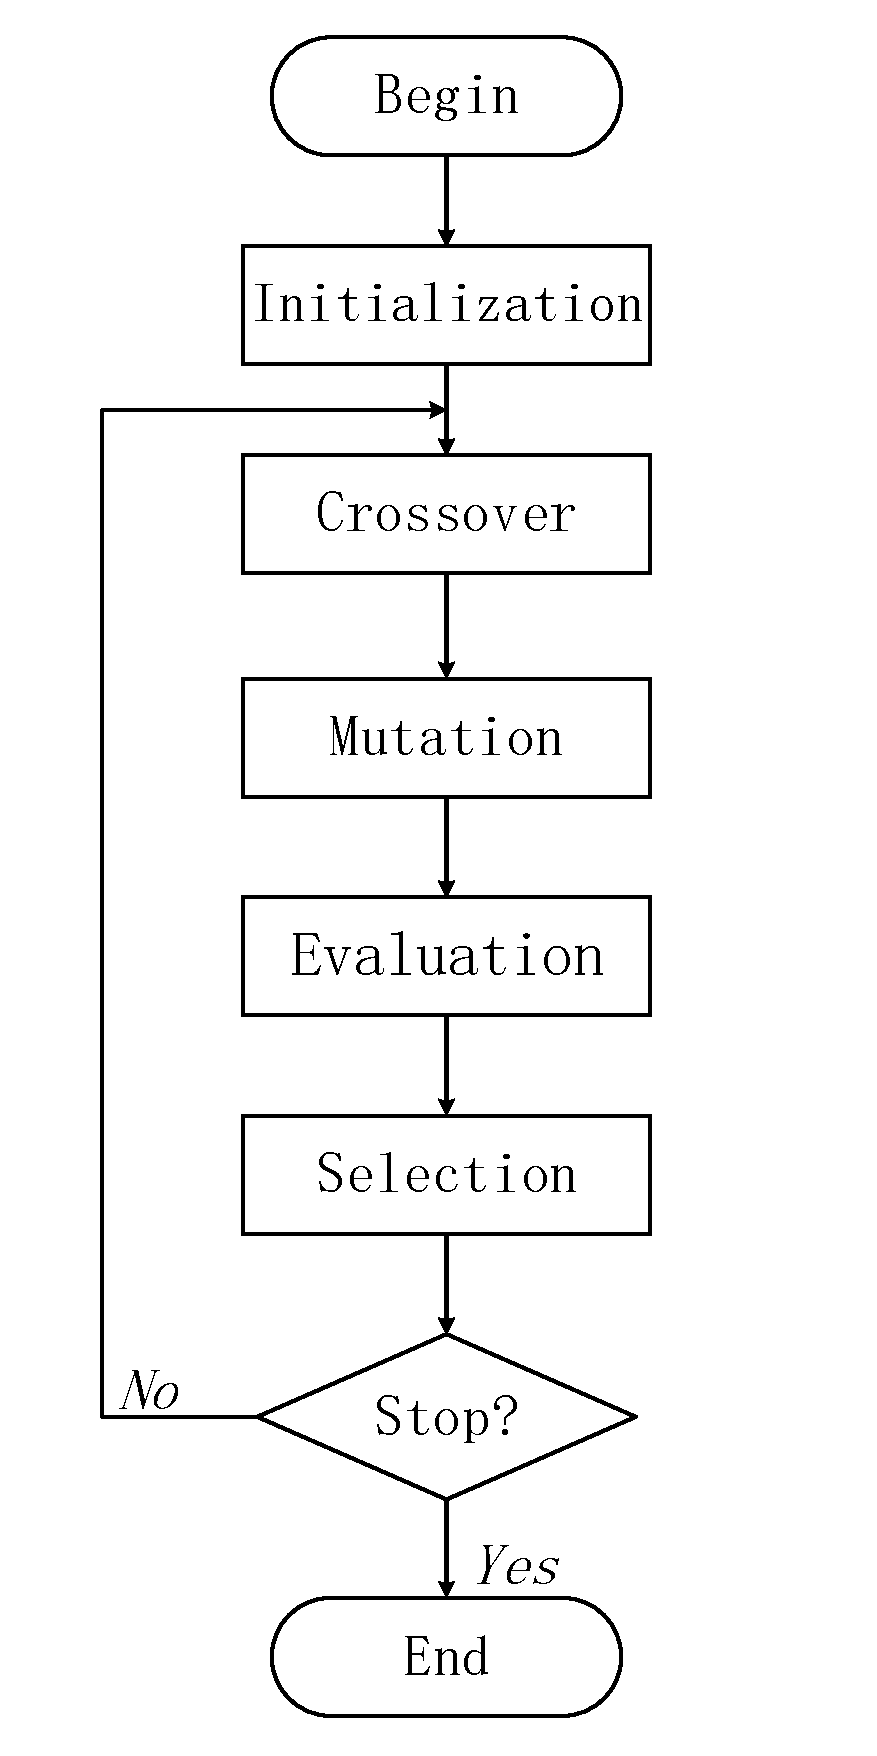
\includegraphics[width=\textwidth]{figures/ea_flow.pdf}
    }
  \end{minipage}
  % second figure
  \begin{minipage}{0.58\textwidth}
    \centering
    \subfigure[Parallel] {
      \label{fig:flow:p}
      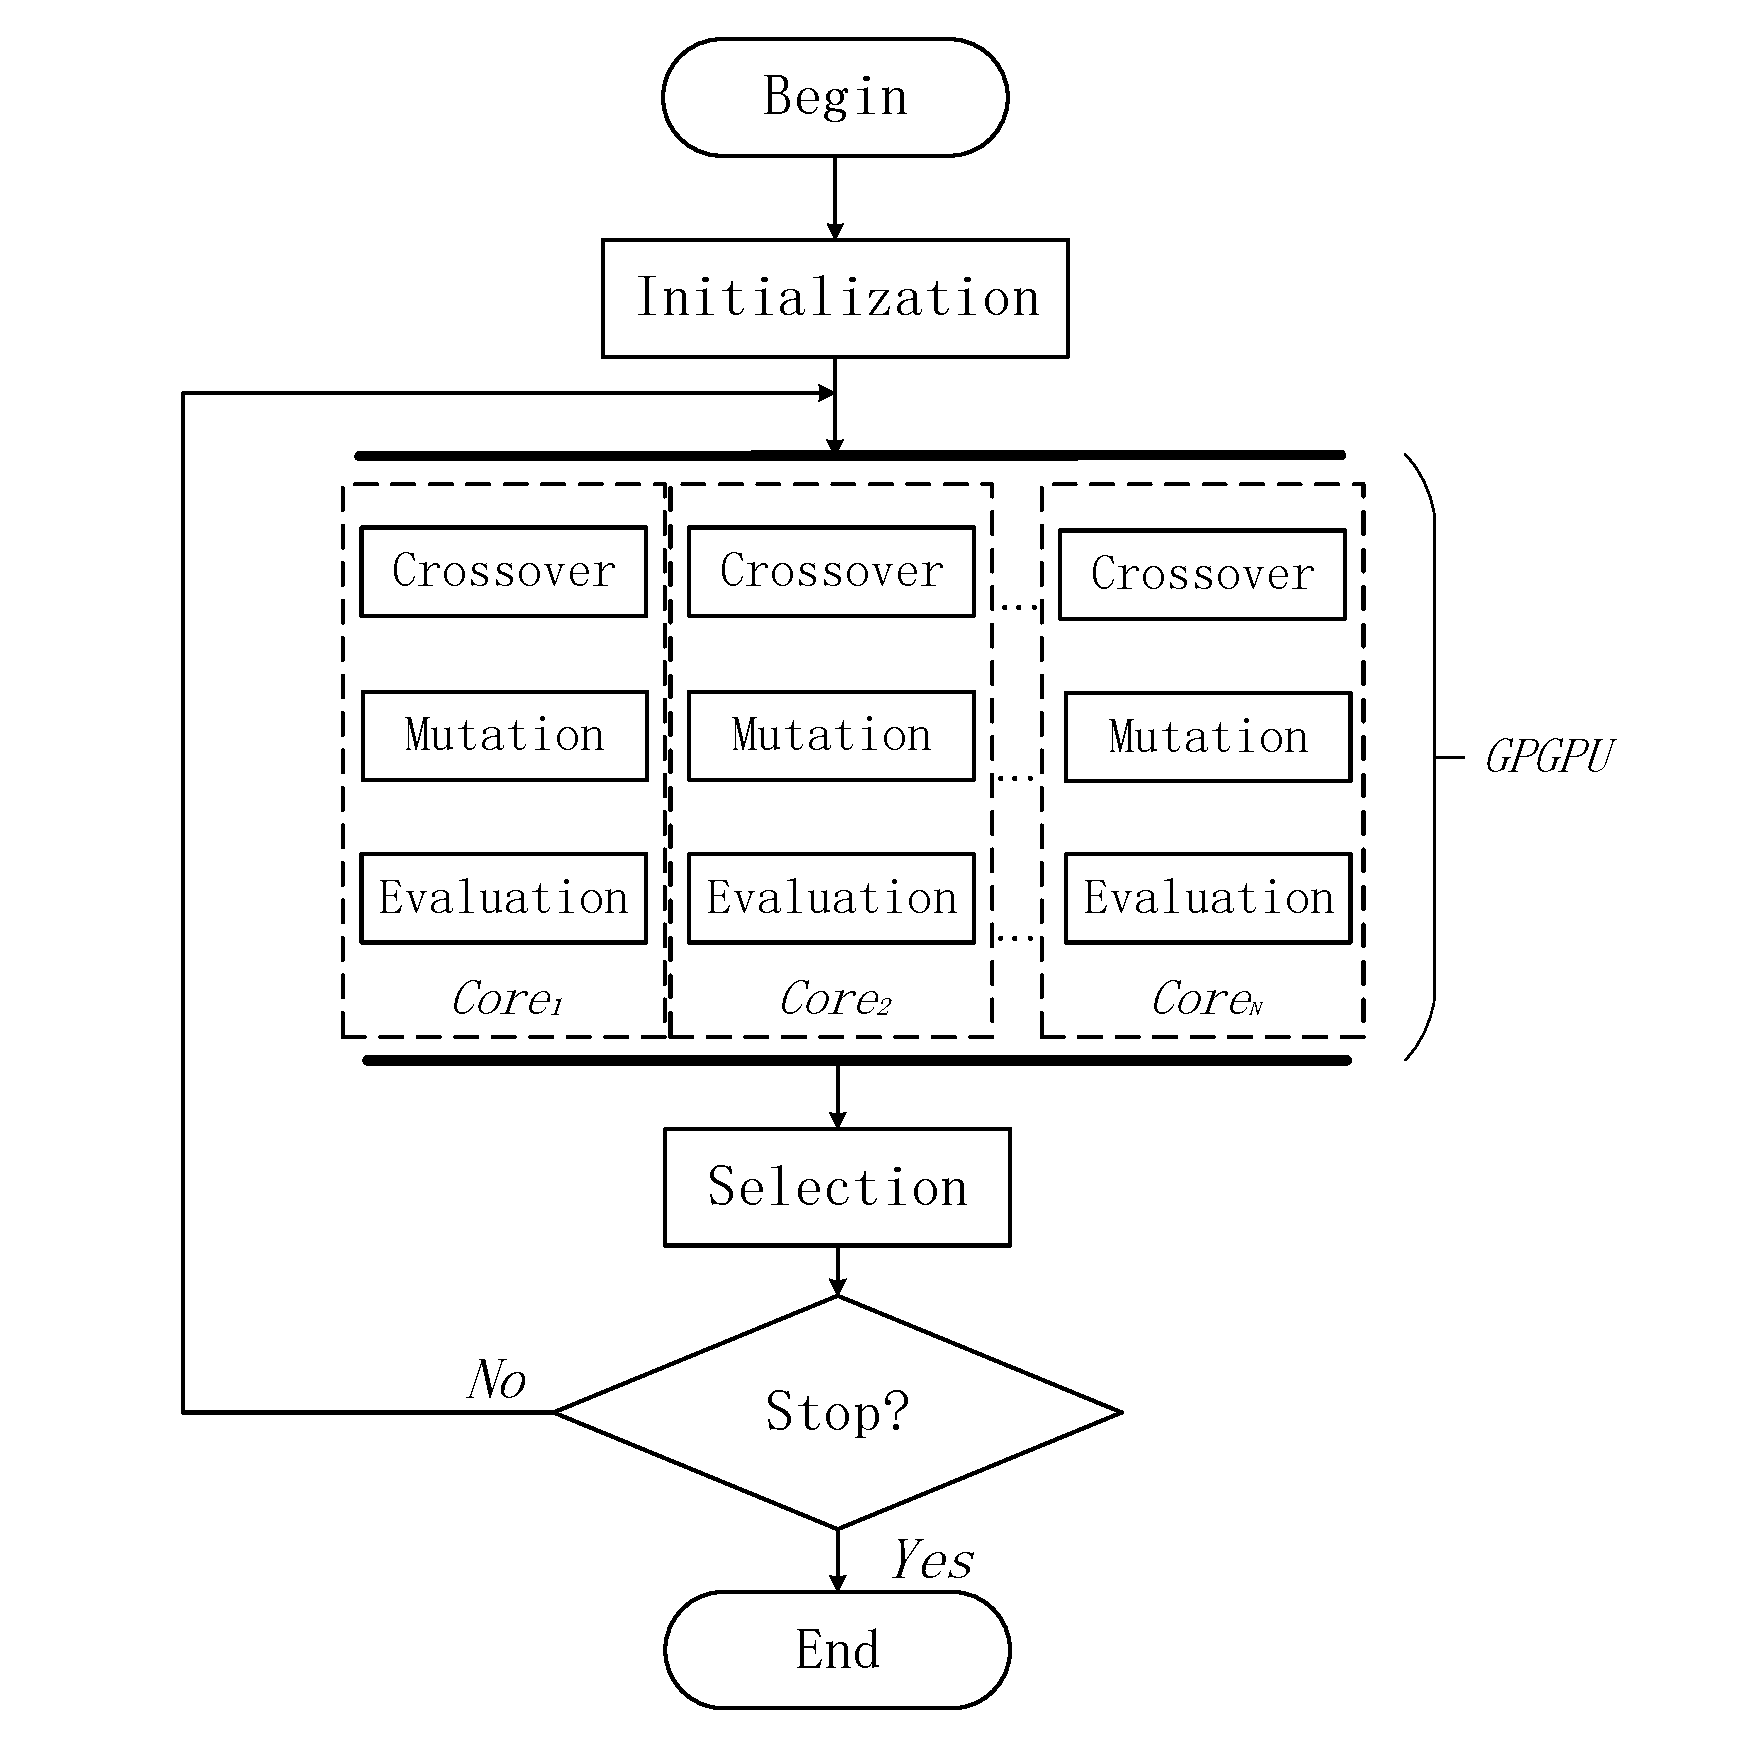
\includegraphics[width=\textwidth]{figures/ea2_flow.pdf}
    }
  \end{minipage}
        \vspace{-2mm}
  \caption{Sequential and Parallel Evolutionary Algorithm}
    \vspace{-7mm}
    \label{fig:flow}
\end{figure}
%\vspace{-10mm}

% !TEX root = ../paper.tex
%
% ---------- chapter 5 ----------
%
% define project name notation
\newcommand{\projectA}[0]{\emph{A-Input}}
\newcommand{\projectB}[0]{\emph{B-DBUpgrade}}
\newcommand{\projectC}[0]{\emph{C-SmartPrice}}

  \vspace{-2mm}
\section{Experimental Results}
  \vspace{-2mm}
To assess the evolutionary algorithm proposed in this paper, two separated
evaluation experiments are made for the effectiveness of evolutionary algorithm
and the efficiency of parallel evolutionary algorithm in project management
problem. The purpose of the experiment is to address the following two
research questions:

\textbf{RQ1}: Does the evolutionary algorithm effectively optimize project
management problem, and get an optimized solution?

\textbf{RQ2}: Is the parallel evolutionary algorithm able to improve the
efficiency in the project management problem?

  \vspace{-2mm}
\subsection{Industrial Project Data}
%
Three industrial project plans have been used in the experimental studies for
this paper, which are named as \projectA{}, \projectB{} and \projectC{}. These
data come from real world projects and have fundamental details, such as work
packages, resources and dependencies. Table \ref{tab:statis} shows the number of
each project.

% 
\begin{table}[!h]
\vspace{-6mm}
  \centering
  \caption{Three Project's Parameters}
        \vspace{-2mm}
  \label{tab:statis}
  \begin{tabular}{lccc}
    \hline
      & $\#$ work packages & $\#$ resources & $\#$ dependencies \\
    \hline
    \projectA{} & 33  & 4  & 33  \\
    \projectB{} & 106 & 8  & 105 \\
    \projectC{} & 74  & 14 & 73  \\
    \hline
  \end{tabular}
  \vspace{-6mm}
\end{table}

\projectA{} is a simulated small-scale project planning. it is a team work plan
for finishing class assignments. \projectB{} is a real software development
plan, which's goal is to upgrade the Oracle database from the \emph{9g} version
to the \emph{10g} version. \projectB{} is Oracle's non-public version of the
project planning. There were different layers of the organisation involved
including DBAs, BSAs, developers and users.  Furthermore, the project also
included the training of the staff for the new features of the
system. \projectC{} consists of a supply chain enhancement of medium size
affecting mostly the website as well as a few internal applications~\cite{ren2}.

Figure \ref{fig:dag} illustrates the relationship between work packages and
resources. In each sub-figure, the rectangle represents a work package in the
project plan, the content in the rectangle is the work packages' ID and
duration; the arrows between work packages suggest dependencies, notice that
some redundant dependencies is removed; the folders in the bottom are some
certain types of resources that can be allocated to work packages. 

\begin{figure}[!ht]
  \centering
  \subfigure[\projectA{}, $33$ work packages, $4$ resources and $33$ dependencies]{
    \centering
    \label{fig:dag:a} 
    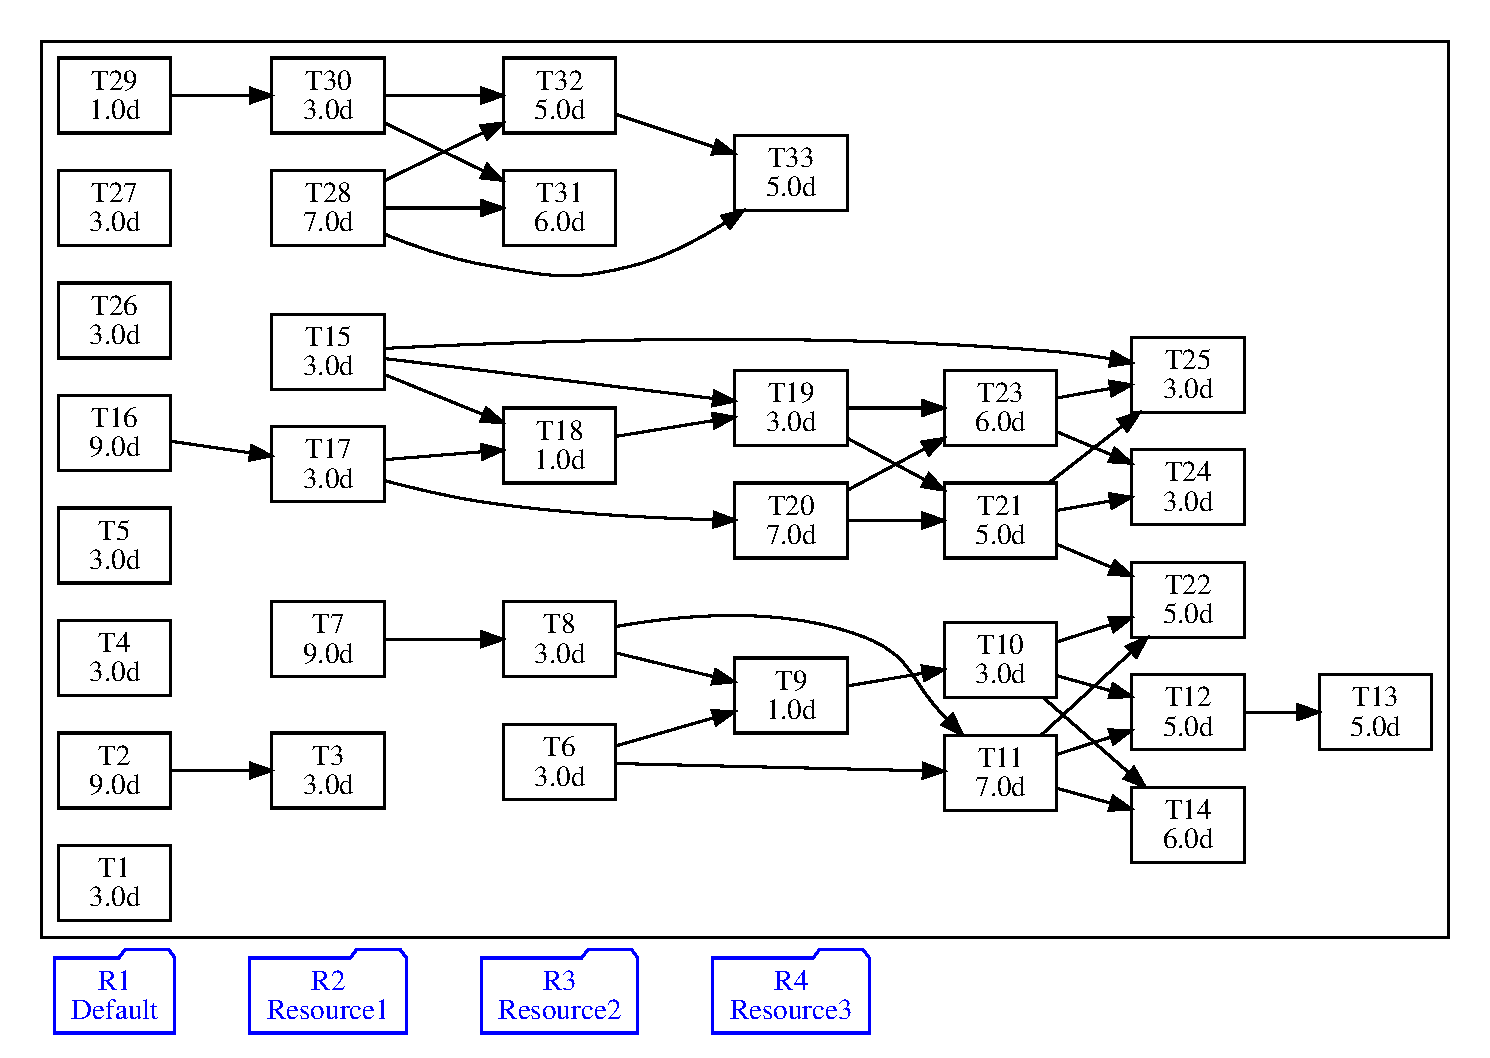
\includegraphics[width=0.75\textwidth]{figures/a.eps}
  }
  \subfigure[\projectB{}: $106$ work packages, $8$ resources and $105$ dependencies]{
    \centering
    \label{fig:dag:b}
    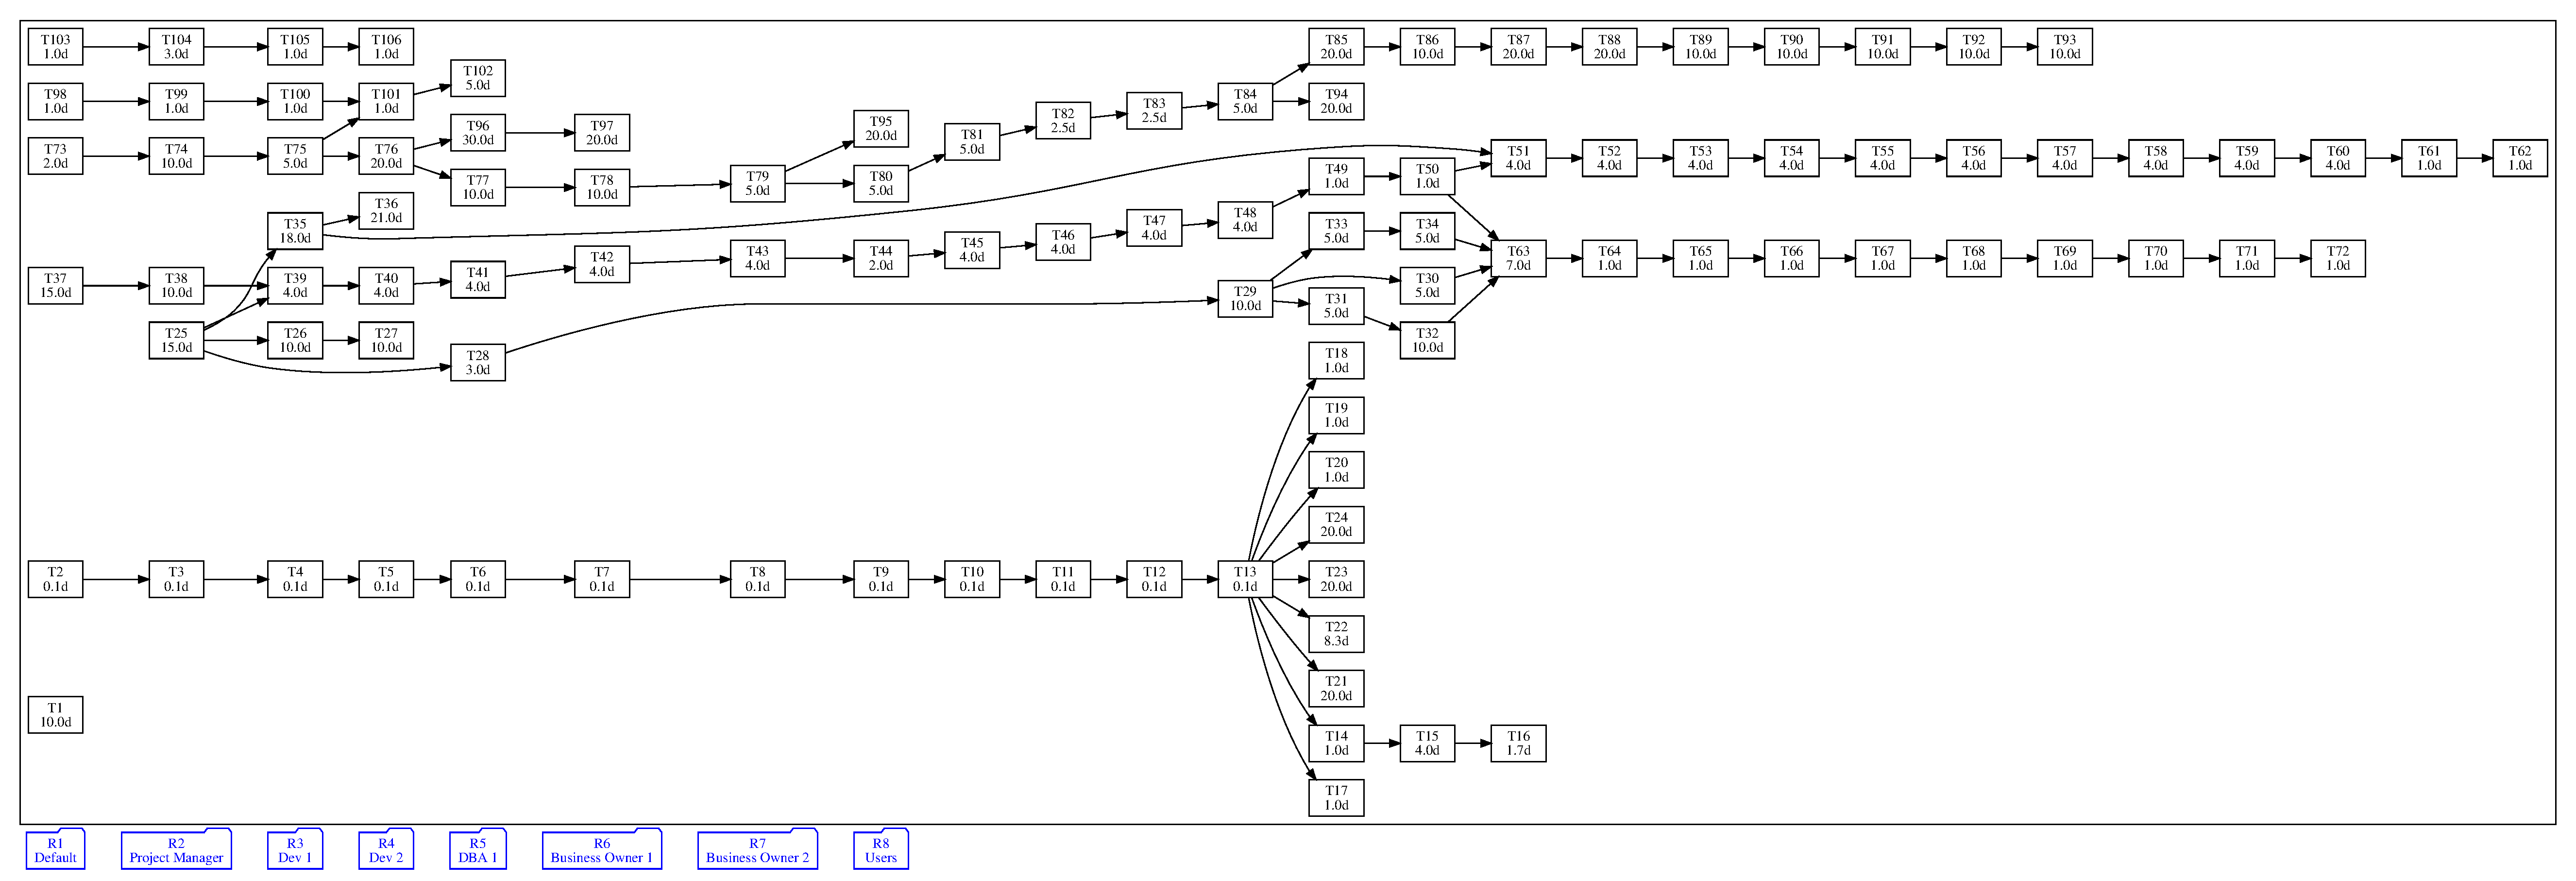
\includegraphics[width=\textwidth]{figures/b.eps}
  }
  \subfigure[\projectC{}:, $74$ work packages, $14$ resources and $73$ dependencies]{
    \centering
    \label{fig:dag:c}
    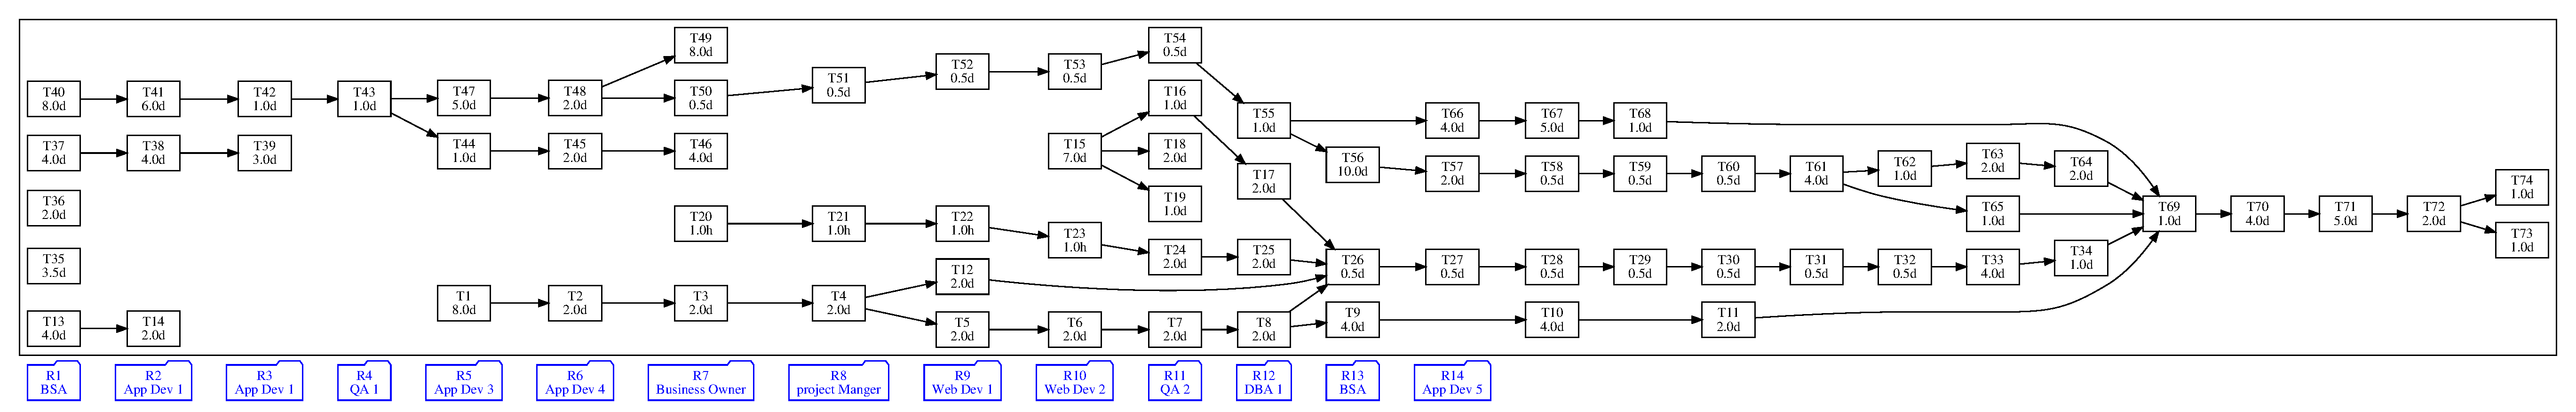
\includegraphics[width=\textwidth]{figures/c.eps}
  }
        \vspace{-5mm}
  \caption{Three Projects' \emph{work packages}, \emph{resources} and \emph{dependencies}}
  \label{fig:dag}
  \vspace{-5mm}
\end{figure}


\subsection{Effectiveness Experiment for Algorithm}
%
In order to answer \textbf{RQ1}, this section designs an effectiveness experiment
for evolutionary algorithm. The basic configuration used in the experiment is
that $100$ individuals runs in $50$ generations. For each generation in the
evolutionary algorithm, we evaluate each individuals' fitness value in the
whole population, and then plot the statistical data into a boxplot diagram.

% effectiveness experiment results
\begin{figure}[!h]
  \centering
        \vspace{-2mm}
  \subfigure[\projectA{}'s solution converges on \emph{19th} generation]{
    \label{fig:pj:a} 
    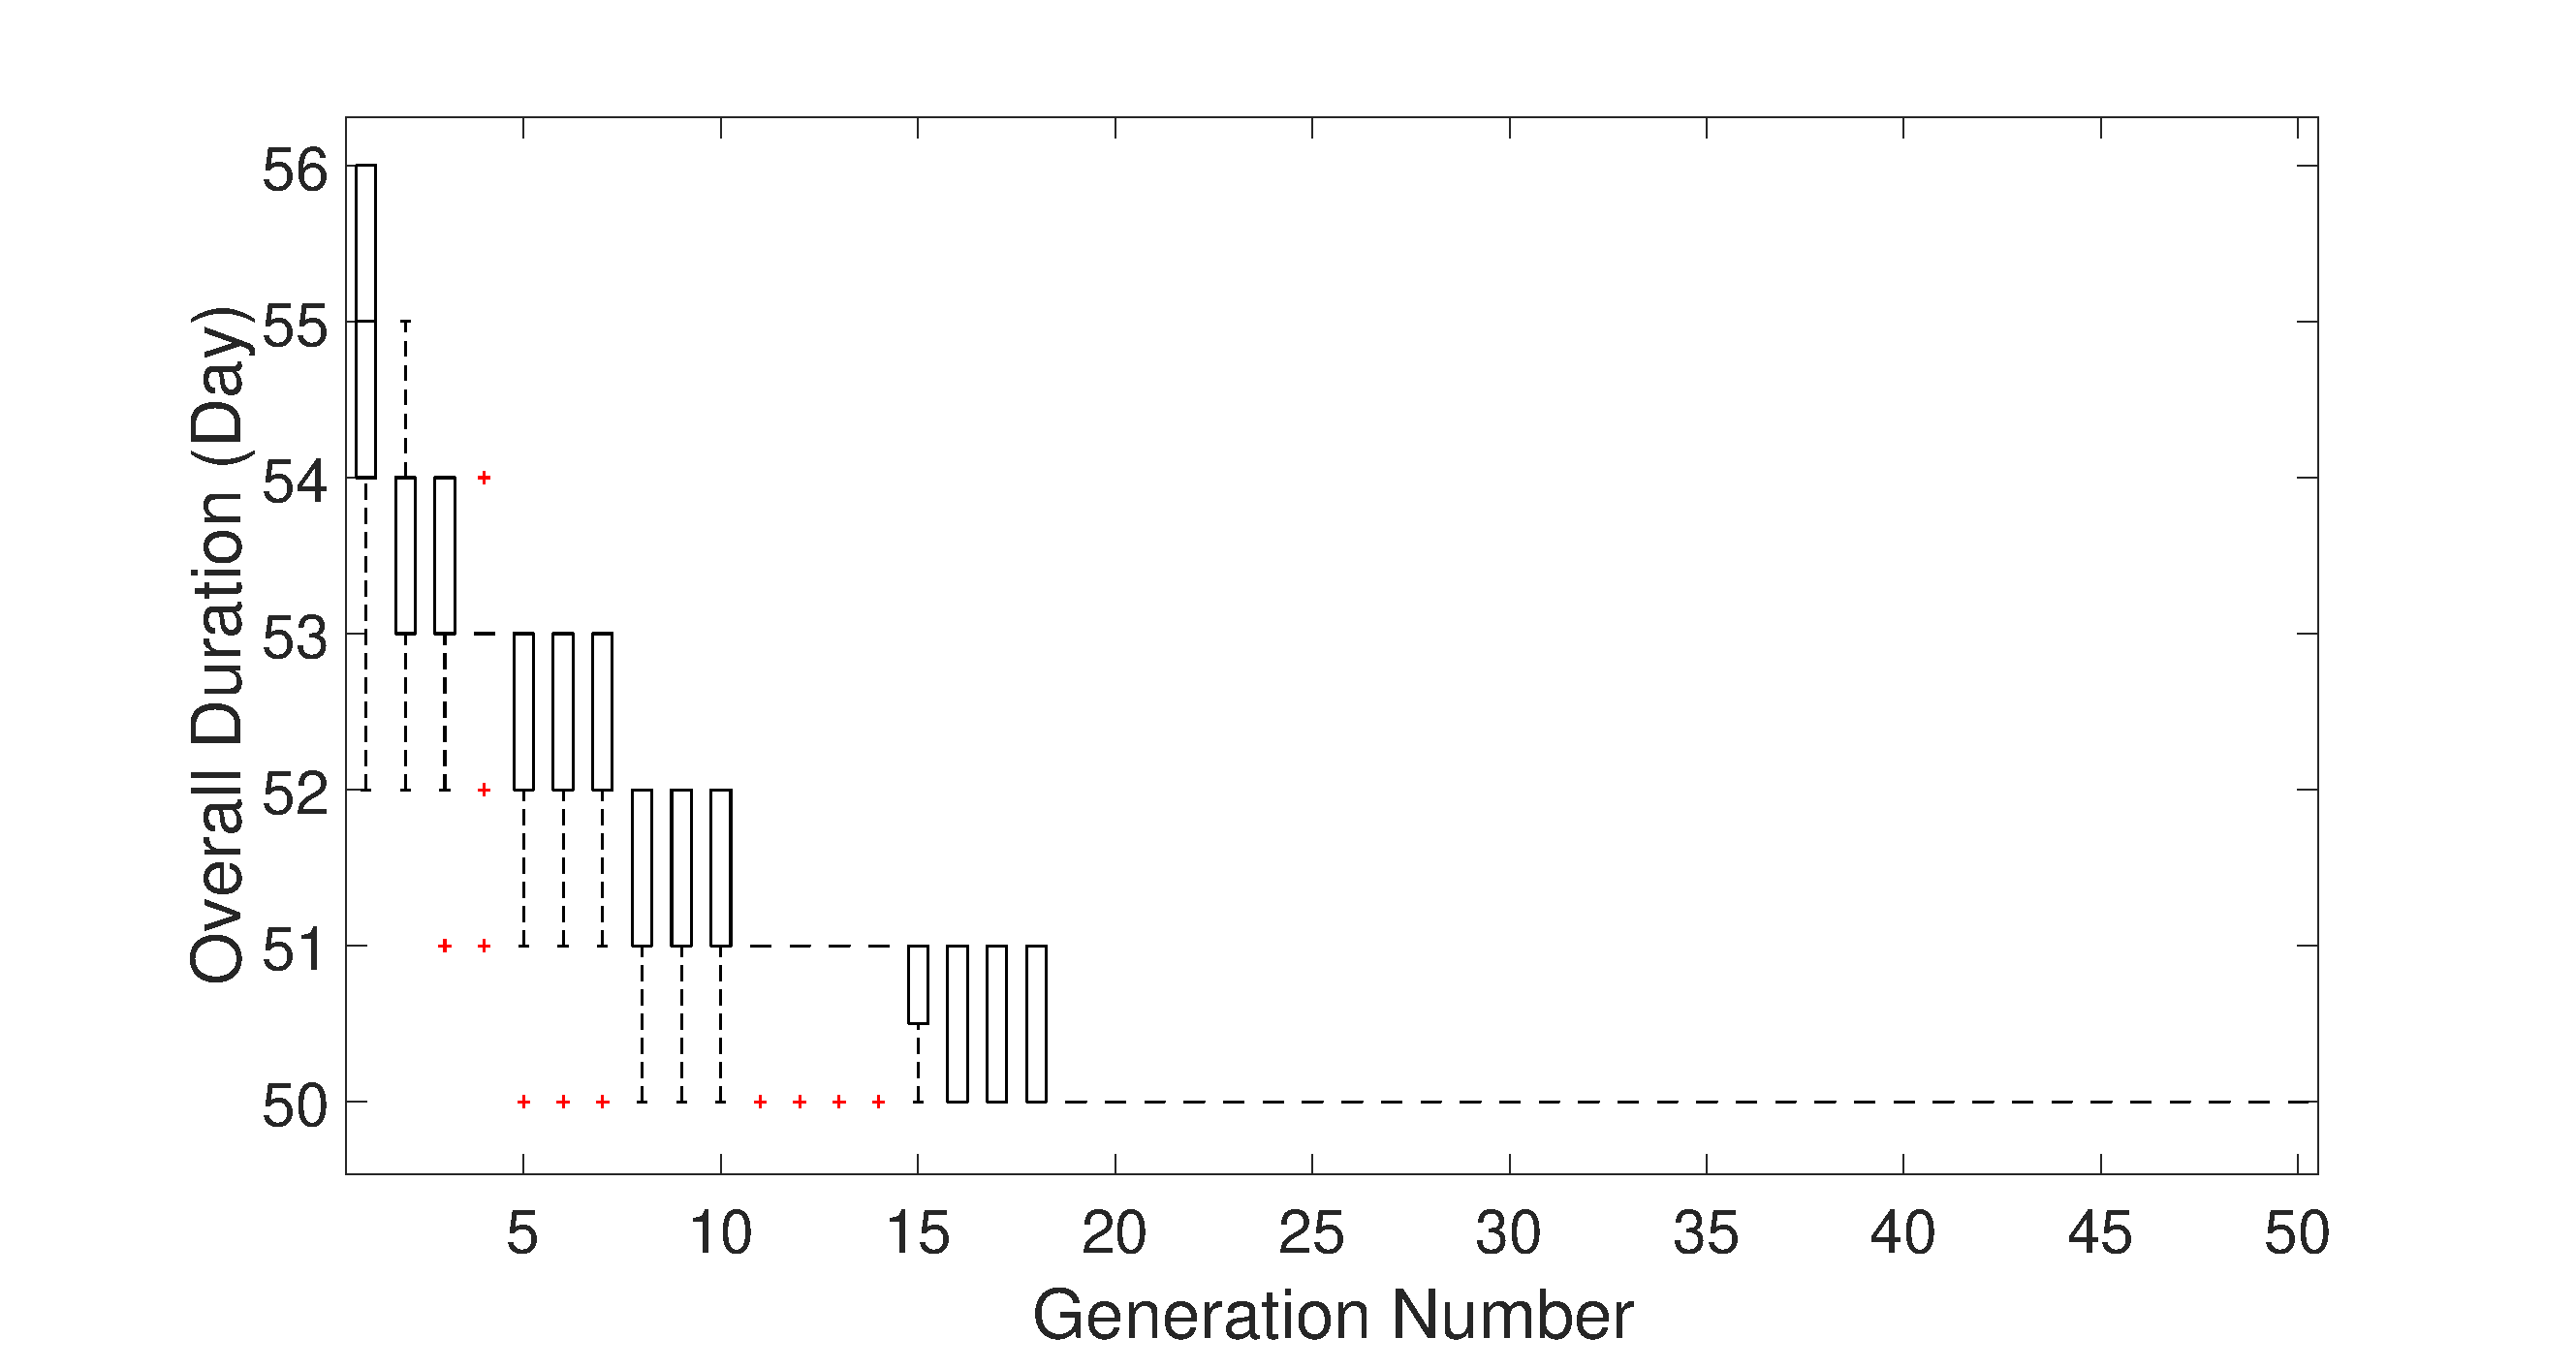
\includegraphics[width=.7\textwidth]{figures/fig_pa1.eps}
  }
      \vspace{-2mm}
  \subfigure[\projectB{}'s solution converges on \emph{22rd} generation]{
    \label{fig:pj:b} 
    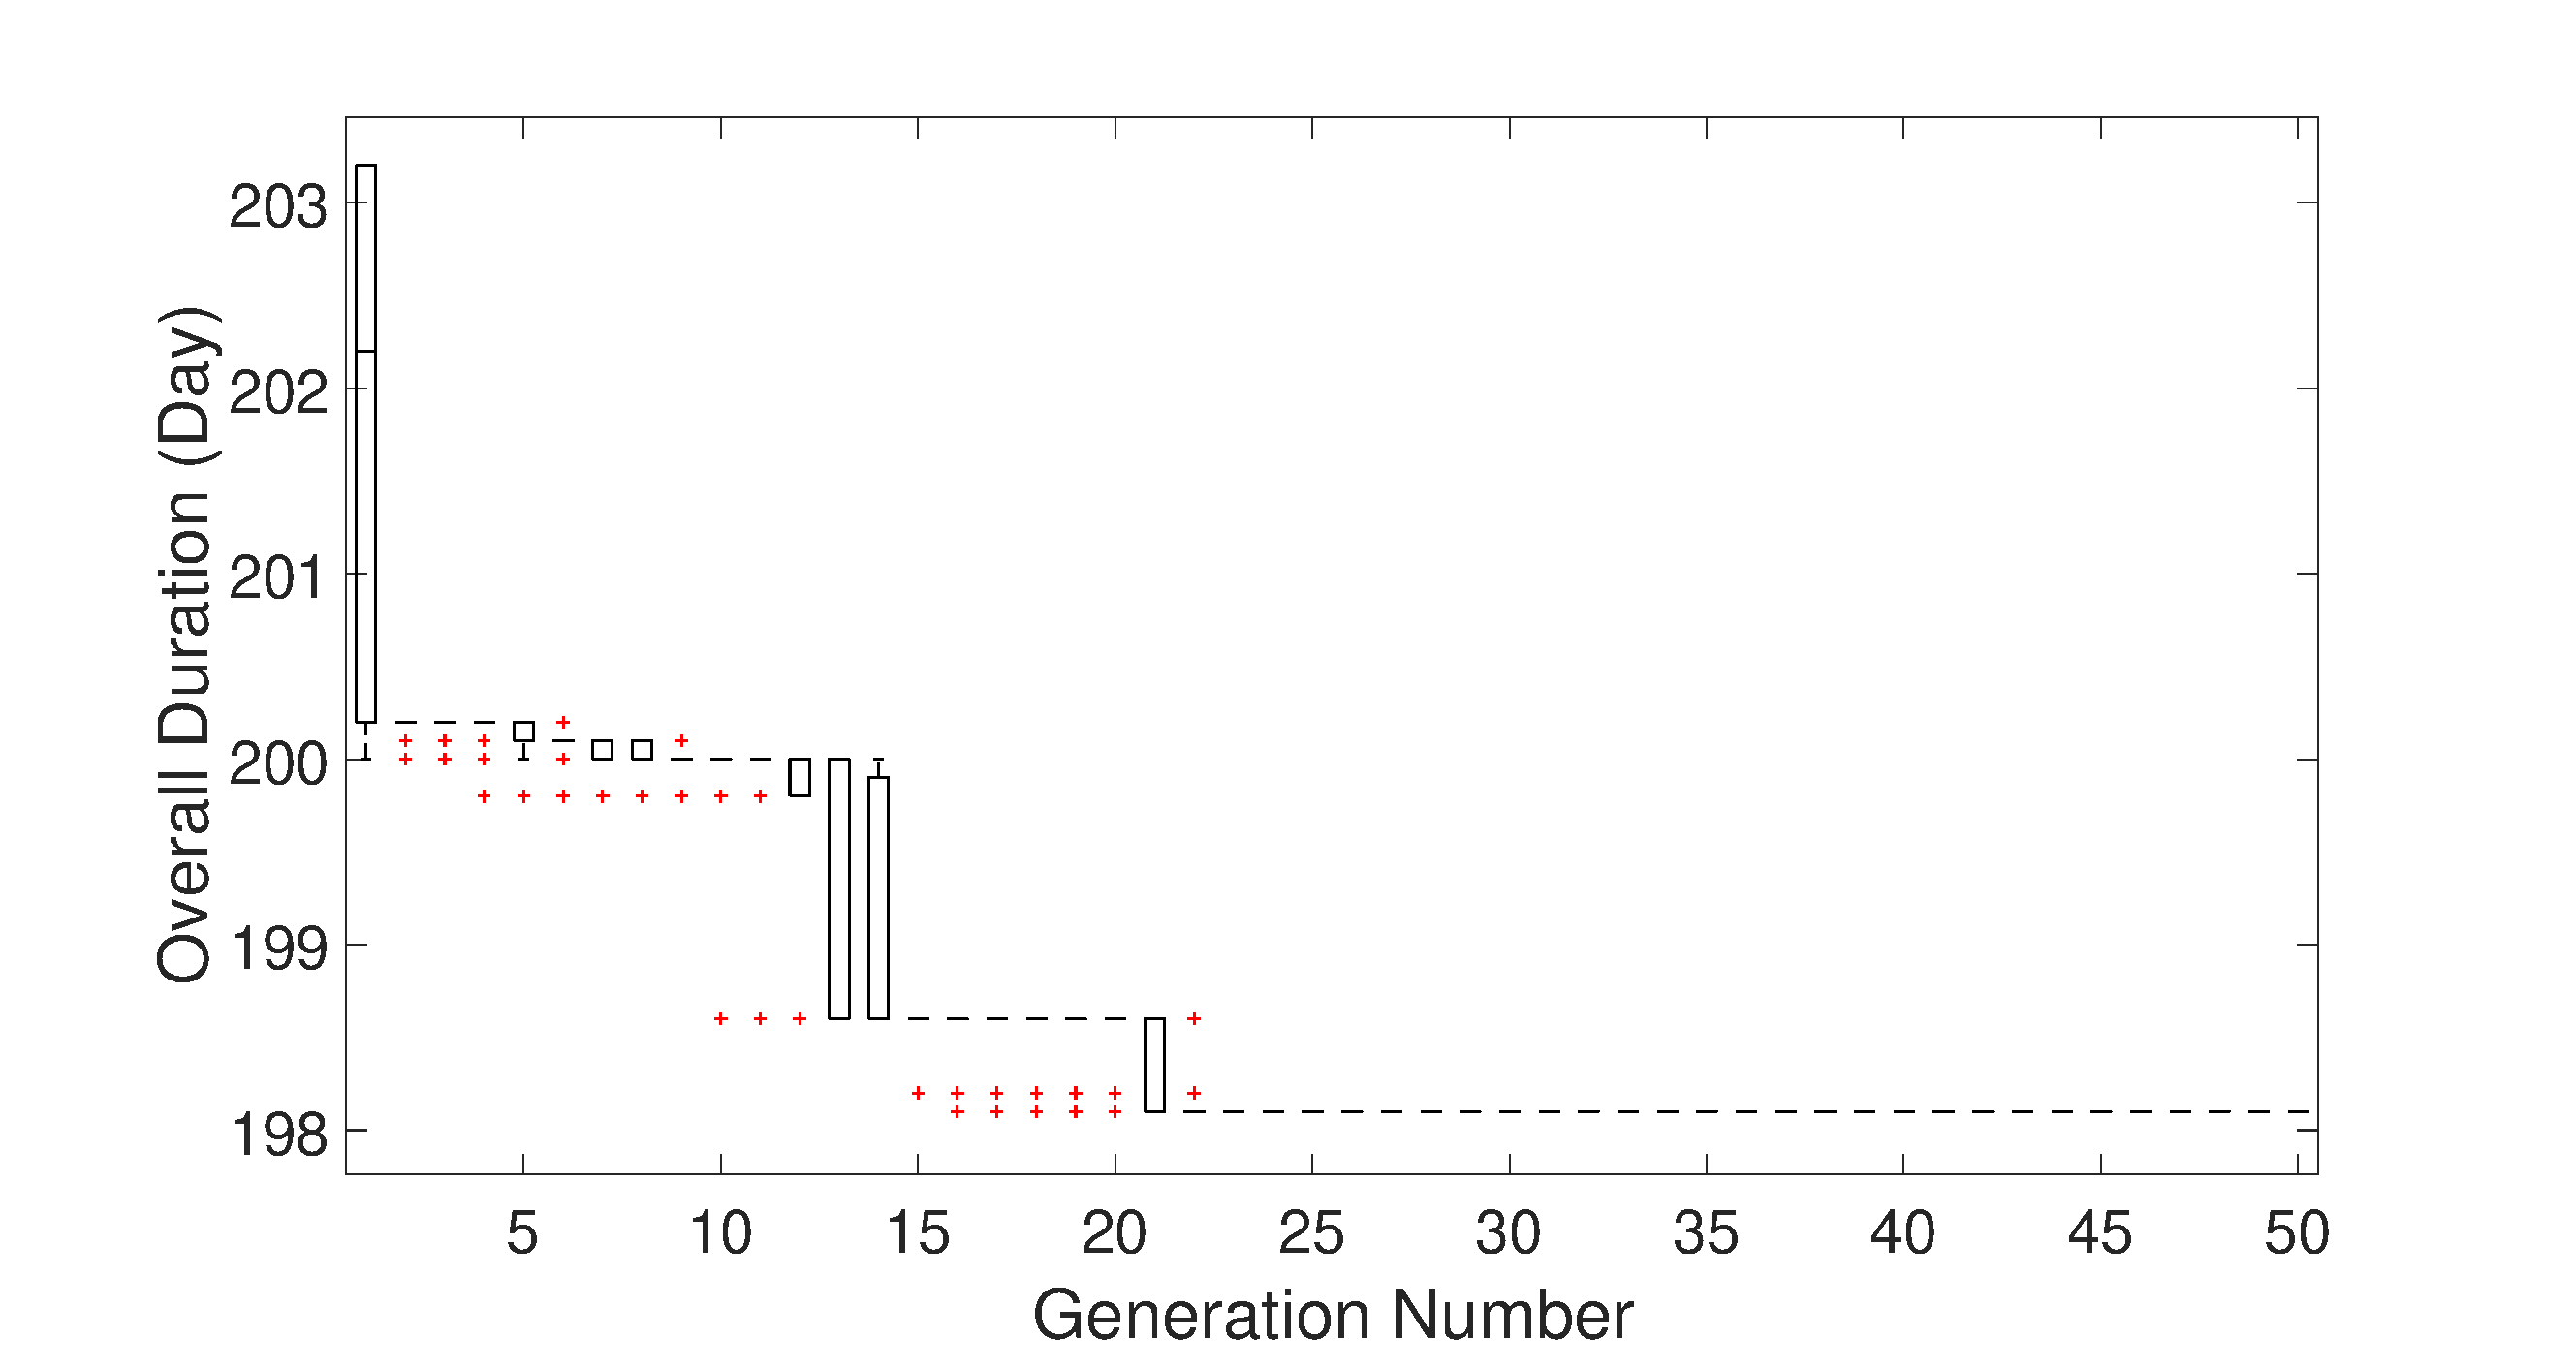
\includegraphics[width=.7\textwidth]{figures/fig_pa2.eps}
  }
        \vspace{-2mm}
  \subfigure[\projectC{}'s solution converges on \emph{15th} generation]{
    \label{fig:pj:c} 
    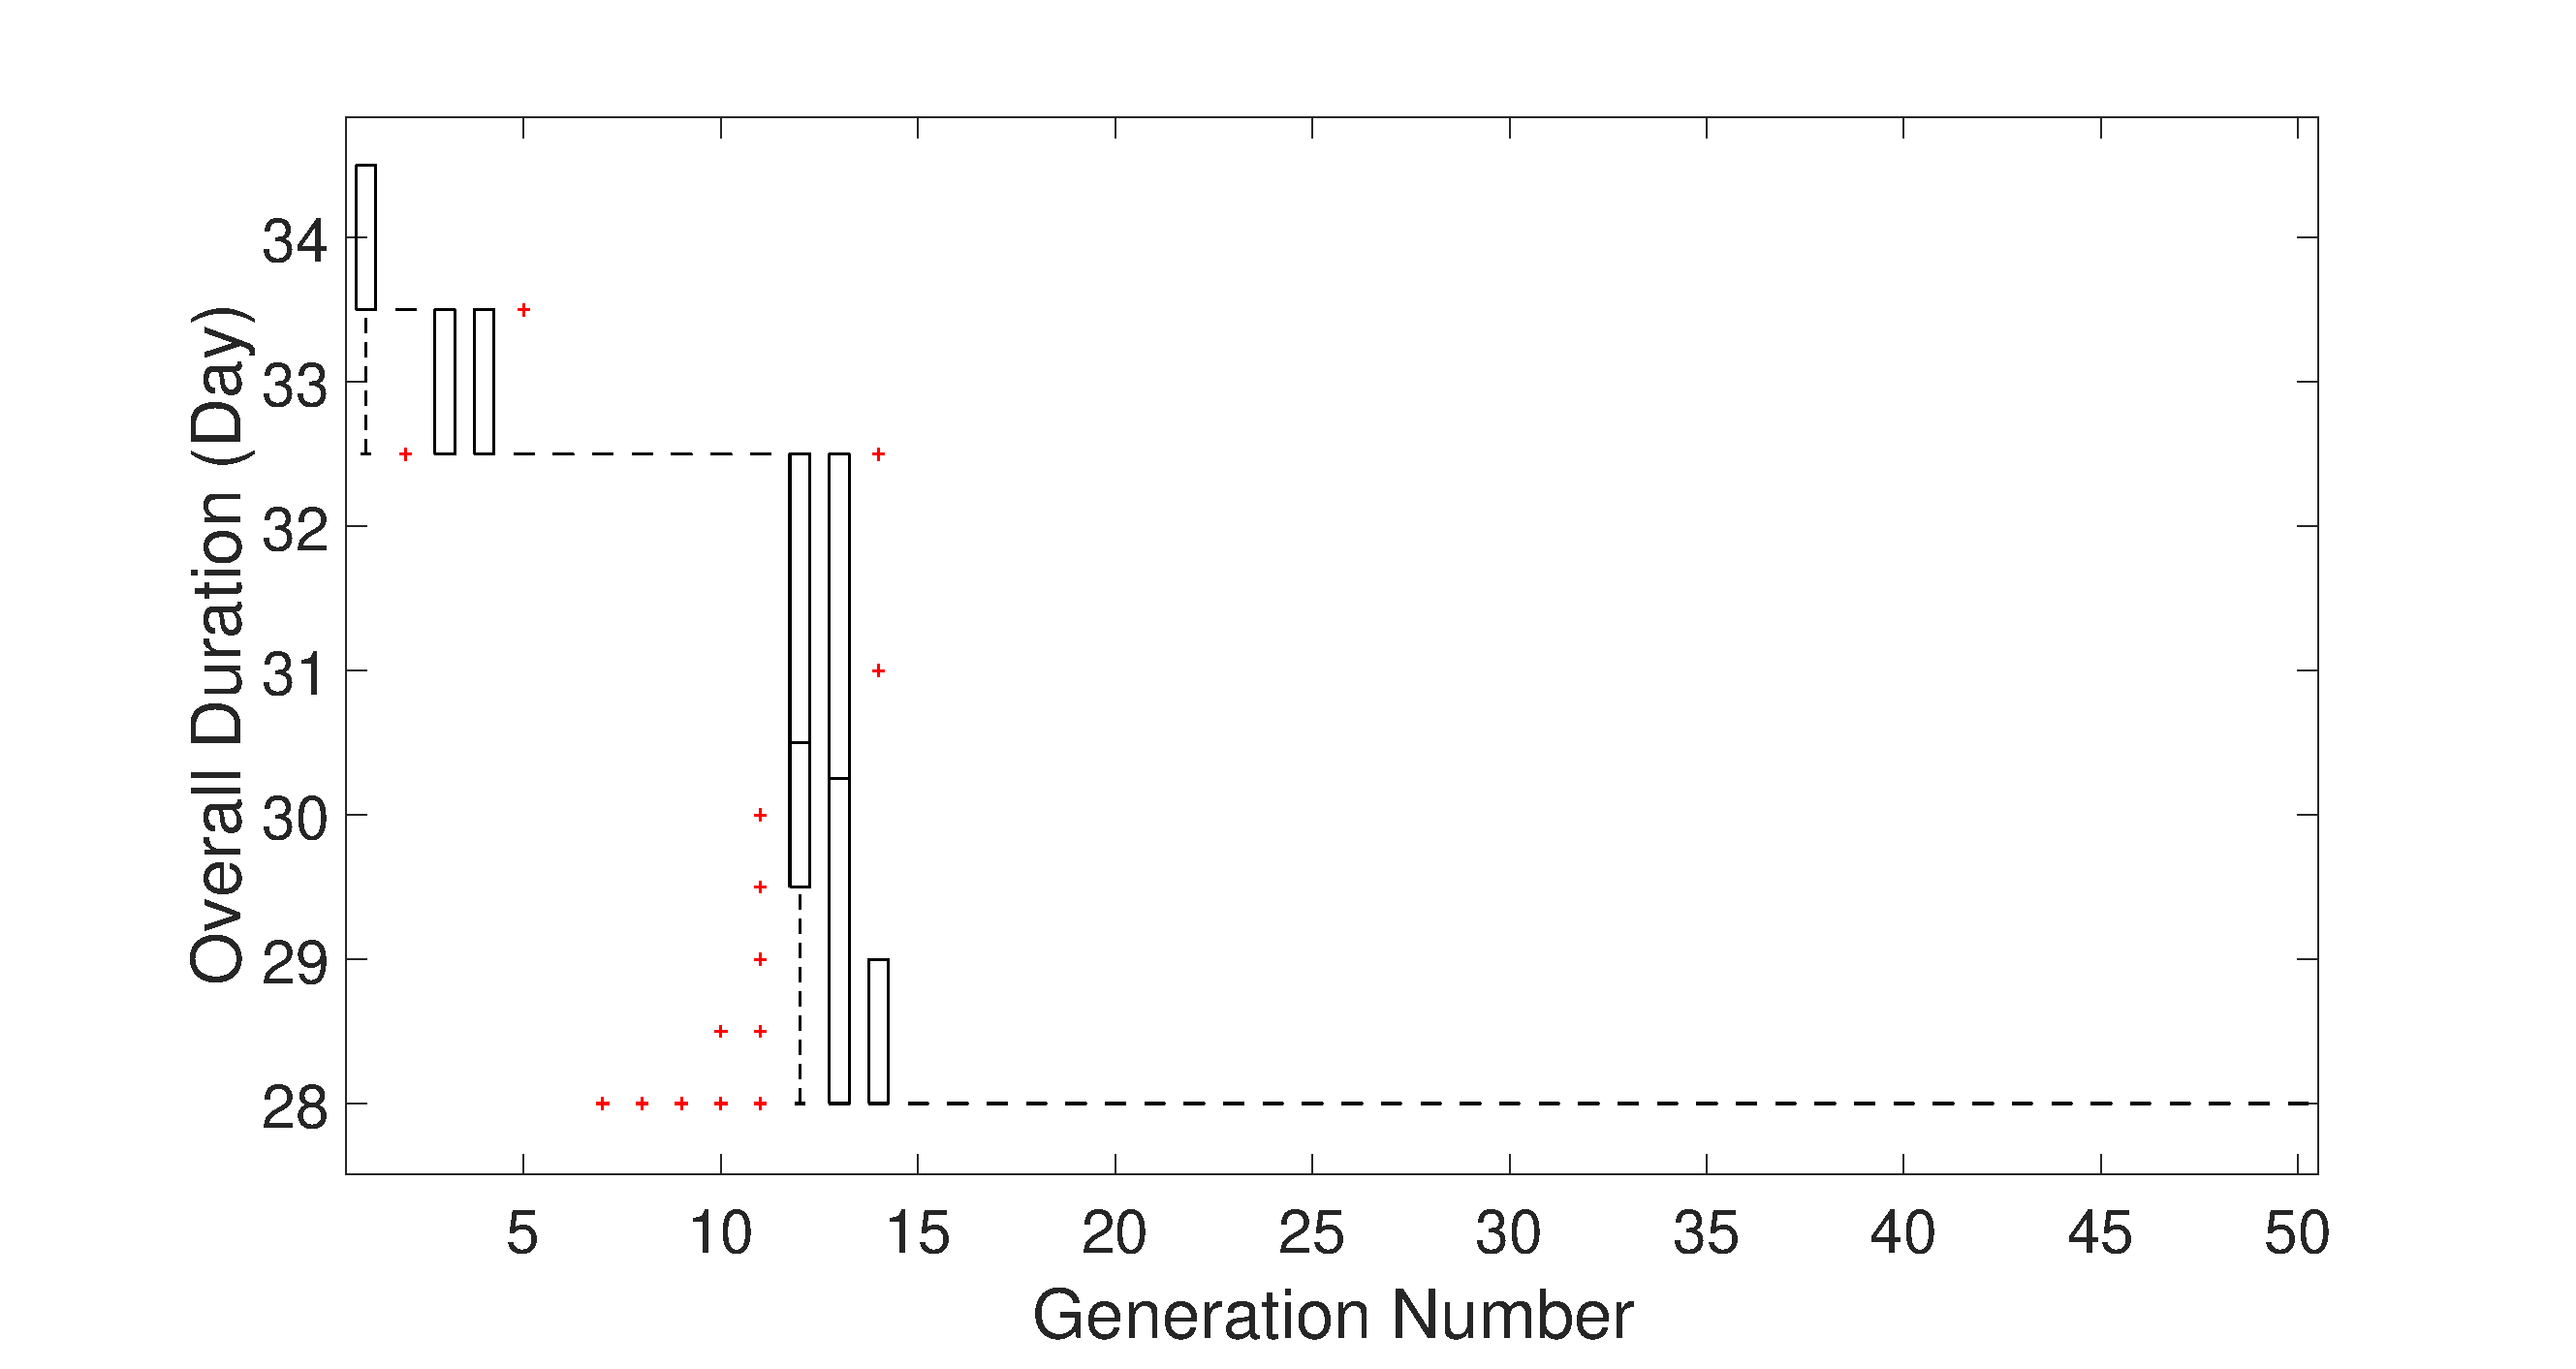
\includegraphics[width=0.7\textwidth]{figures/fig_pa3.eps}
  }
  \caption{Statistics of Fitness Value in Each Generation}
  \label{fig:pj}
  \vspace{-8mm}
\end{figure}

The boxplot diagram shows the five kinds of statistical data of all individuals'
fitness value in each generation. The data are the minimum, the lower quartile,
the median, the upper quartile and the maximum values of the whole
population. Figure \ref{fig:pj} shows the results of the above-mentioned three
industrial projects. In each sub-figure, the tick labels on the horizontal axis
indicate the total number of internal generations that have been carried out,
and also indicates the point at which the algorithm updated the population used
for fitness computation. At each point on the horizontal axis, the entire
population is depicted using a boxplot to give both a sense of the values
obtained for completion time as the evolution progresses and the distribution of
the fitness values in the population. From the trend of three projects in the
figures, it can be seen that the population is diversified when the population
is initialized and as the number of generation increase, all the fitness value
begins to decrease, and finally converges to an optimized result.

The convergence of solutions is quite fast and stable. Figure \ref{fig:pj:a}
shows the solution of \projectA{} converges on 19th generation. Figure
\ref{fig:pj:b} shows the solution of \projectB{} converges on 22rd generation.
Figure \ref{fig:pj:c} shows the solution of \projectC{} converges on 15th
generation. Those results show us evolutionary algorithm will find an optimized
overall duration for specific project plan.

Through the above analysis results of experimental data, we can accurately
answer \textbf{RQ1}. In the project management problems, the evolutionary
algorithm does have a good optimization and improvement.


\subsection{Efficiency Experiment for Algorithm}
%
In order to answer \textbf{RQ2}, this section conducts an efficiency experiment
that compares the efficiency between the parallel evolutionary algorithm and the
sequential one.

%% \begin{table}[!ht]
%%   \centering
%%   \caption{Hardware Configuration Comparison}
%%   \label{tab:cpugpu}
%%   \begin{tabular}{c|c}
%%     \hline
%%     CPU & GPU  \\
%%     \hline
%%     \hspace{.5cm} Intel i7 CPU 870 \hspace{.5cm} & \hspace{.5cm} GeForce GTX 970 \hspace{.5cm} \\
%%     2.93 GHz & 1.27 GHz \\
%%     8 cores & 1664 cores \\
%%     \hline
%%   \end{tabular}
%% \end{table}

\begin{table}[!h]
\vspace{-7mm}
  \centering
  \caption{The Comparison of Sequential and Parallel Implementation}
  \vspace{-3mm}
  \label{tab:time}
  \begin{tabular}{ccc|cc|cc}
    \hline
    & \multicolumn{2}{c}{ \projectA{} } & \multicolumn{2}{c}{ \projectB{} } & \multicolumn{2}{c}{ \projectC } \\
    \hline
      Time(ms) & \hspace{.25cm} CPU \hspace{.25cm} & \hspace{.25cm} GPU \hspace{.25cm} & \hspace{.25cm} CPU \hspace{.25cm} & \hspace{.25cm} GPU \hspace{.25cm} & \hspace{.25cm} CPU \hspace{.25cm} & \hspace{.25cm} GPU \hspace{.25cm}\\
    \hline
     1    & 7991.8 & 4102.5 & 45225.1 & 21217.5 & 29642.9 & 14844.3 \\
     2    & 8431.8 & 4279.7 & 44832.1 & 21377.9 & 28733.7 & 14543.6 \\
     3    & 7504.1 & 3947.9 & 44934.9 & 21227.2 & 28657.9 & 15003.4 \\
     4    & 7442.1 & 4642.5 & 44197.1 & 21340.3 & 29489.5 & 14882.8 \\
     5    & 7376.9 & 4263.8 & 45233.7 & 22448.2 & 29379.5 & 14921.5 \\
     6    & 7385.4 & 4188.6 & 45197.5 & 20956.1 & 28687.9 & 14723.3 \\
     7    & 8238.8 & 4540.2 & 45305.4 & 21777.2 & 29786.3 & 13978.8 \\
     8    & 7470.7 & 4226.4 & 45322.8 & 21147.1 & 31231.7 & 14811.1 \\
     9    & 7604.8 & 3778.2 & 45040.7 & 21004.7 & 28319.7 & 14292.0 \\
     10   & 7451.9 & 4712.4 & 45970.6 & 21500.9 & 28322.1 & 14429.7 \\
    \hline
     Avg. & 7689.8 & 4268.2 & 45126.0 & 21399.7 & 29225.1 & 14643.1 \\
    \hline
  \end{tabular}
  \vspace{-7mm}
\end{table}


The initial configuration of the two algorithms is the identical, which the
number of population is $1000$ and the number of generation is $100$. Each
generation runs several steps including crossover, mutation and selection etc. A
timer is set to record the total executing time of the experiments. The timer
starts after loading initial data and ends after the result is calculated. This
operation allows us to count the real executing time both in the sequential
environment and the parallel environment under the same criteria. The efficiency
experiments are repeated $10$ times. Table \ref{tab:time} shows the comparison
of sequential and parallel implementation executing time on all three industrial
projects. By the comparison of average executing time of $10$ times results, the
average executing time of \projectA{} on CPU is $1.80$ times than GPU, the
average executing time of \projectB{} on CPU is $2.10$ times than GPU and the
average executing time of \projectC{} on CPU is $2.00$ times than GPU.

In summary, the executing time of sequential algorithm on CPU is roughly twice
as long as the parallel algorithm on GPU. So it can be a good answer to
\textbf{RQ2} that parallel evolutionary algorithm can improve the efficiency on
computing the project management problems.

%% The final result of \projectA{}, \projectB{} and \projectC{} are
%% shown in figures \ref{fig:co}. It can be seen from the figures that the
%% time-consuming of the sequential algorithm on CPU is roughly twice as long as
%% the parallel algorithm on GPU.


% comparison figures
%% \begin{figure}[!hb]
%%   \centering
%%   \subfigure[\projectA{}'s executing time spend on CPU is \emph{1.80} times than GPU]{
%%     \label{fig:co:a}
%%     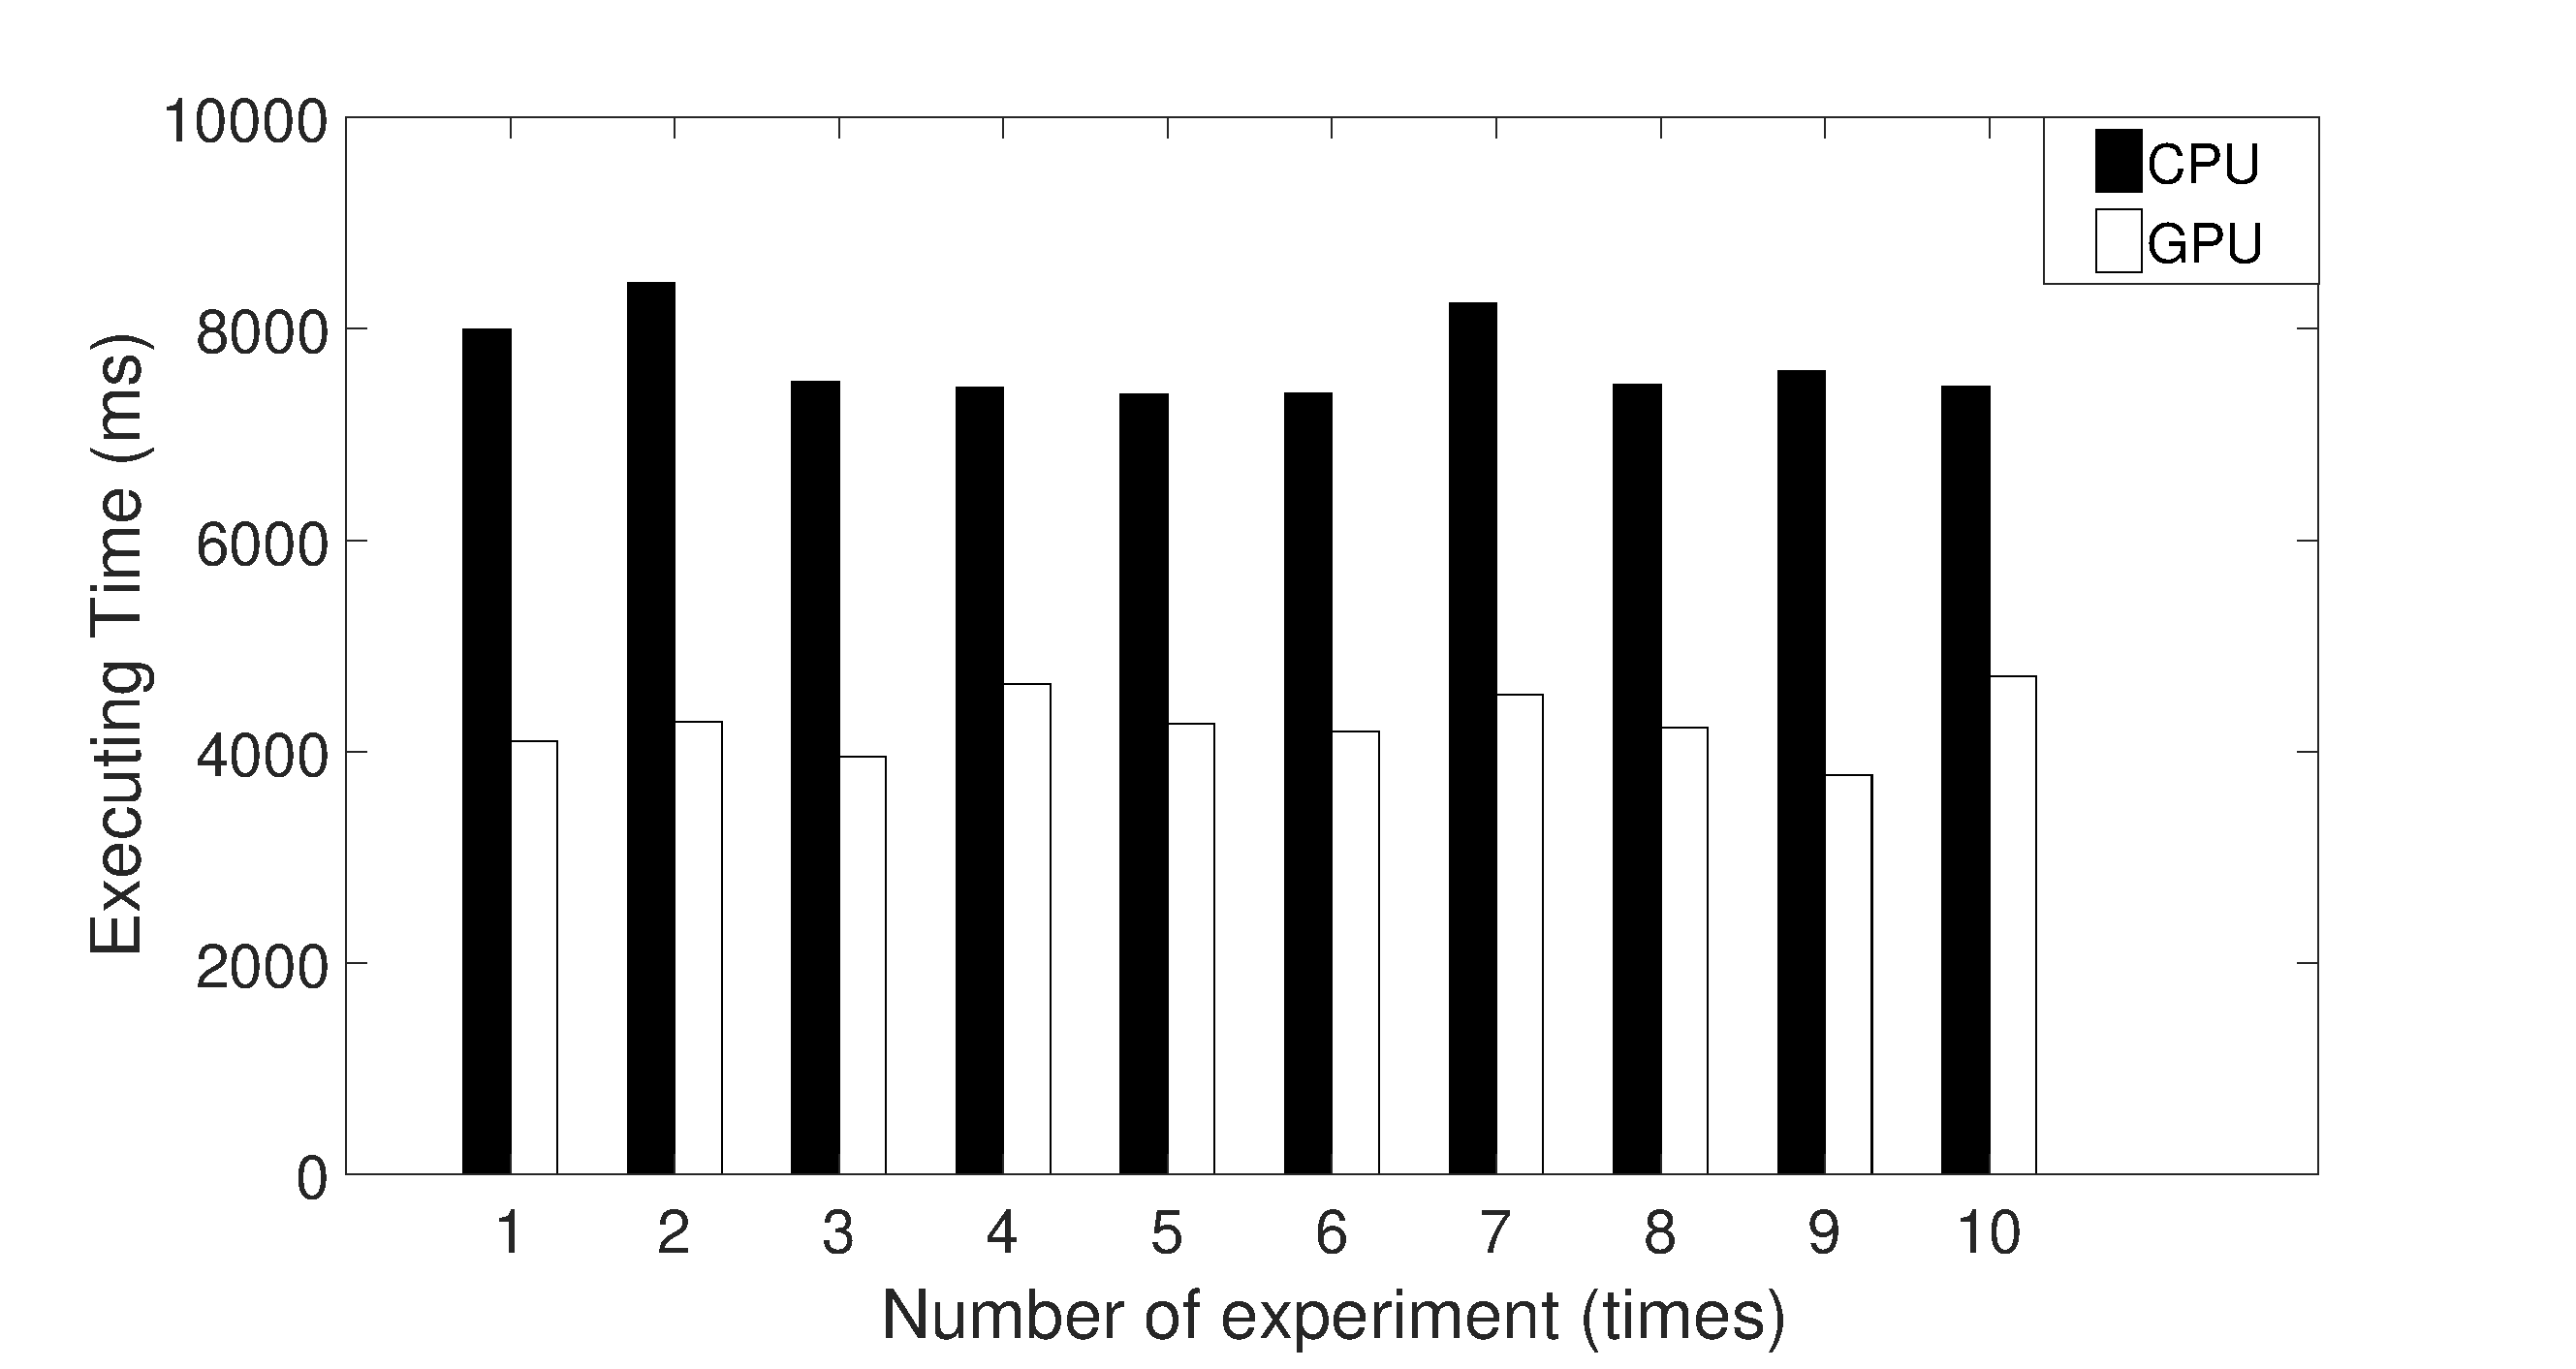
\includegraphics[width=0.8\textwidth]{figures/fig_co1.eps} }
%%   \subfigure[\projectB{}'s executing time spend on CPU is \emph{2.10} times than GPU]{
%%     \label{fig:co:b}
%%     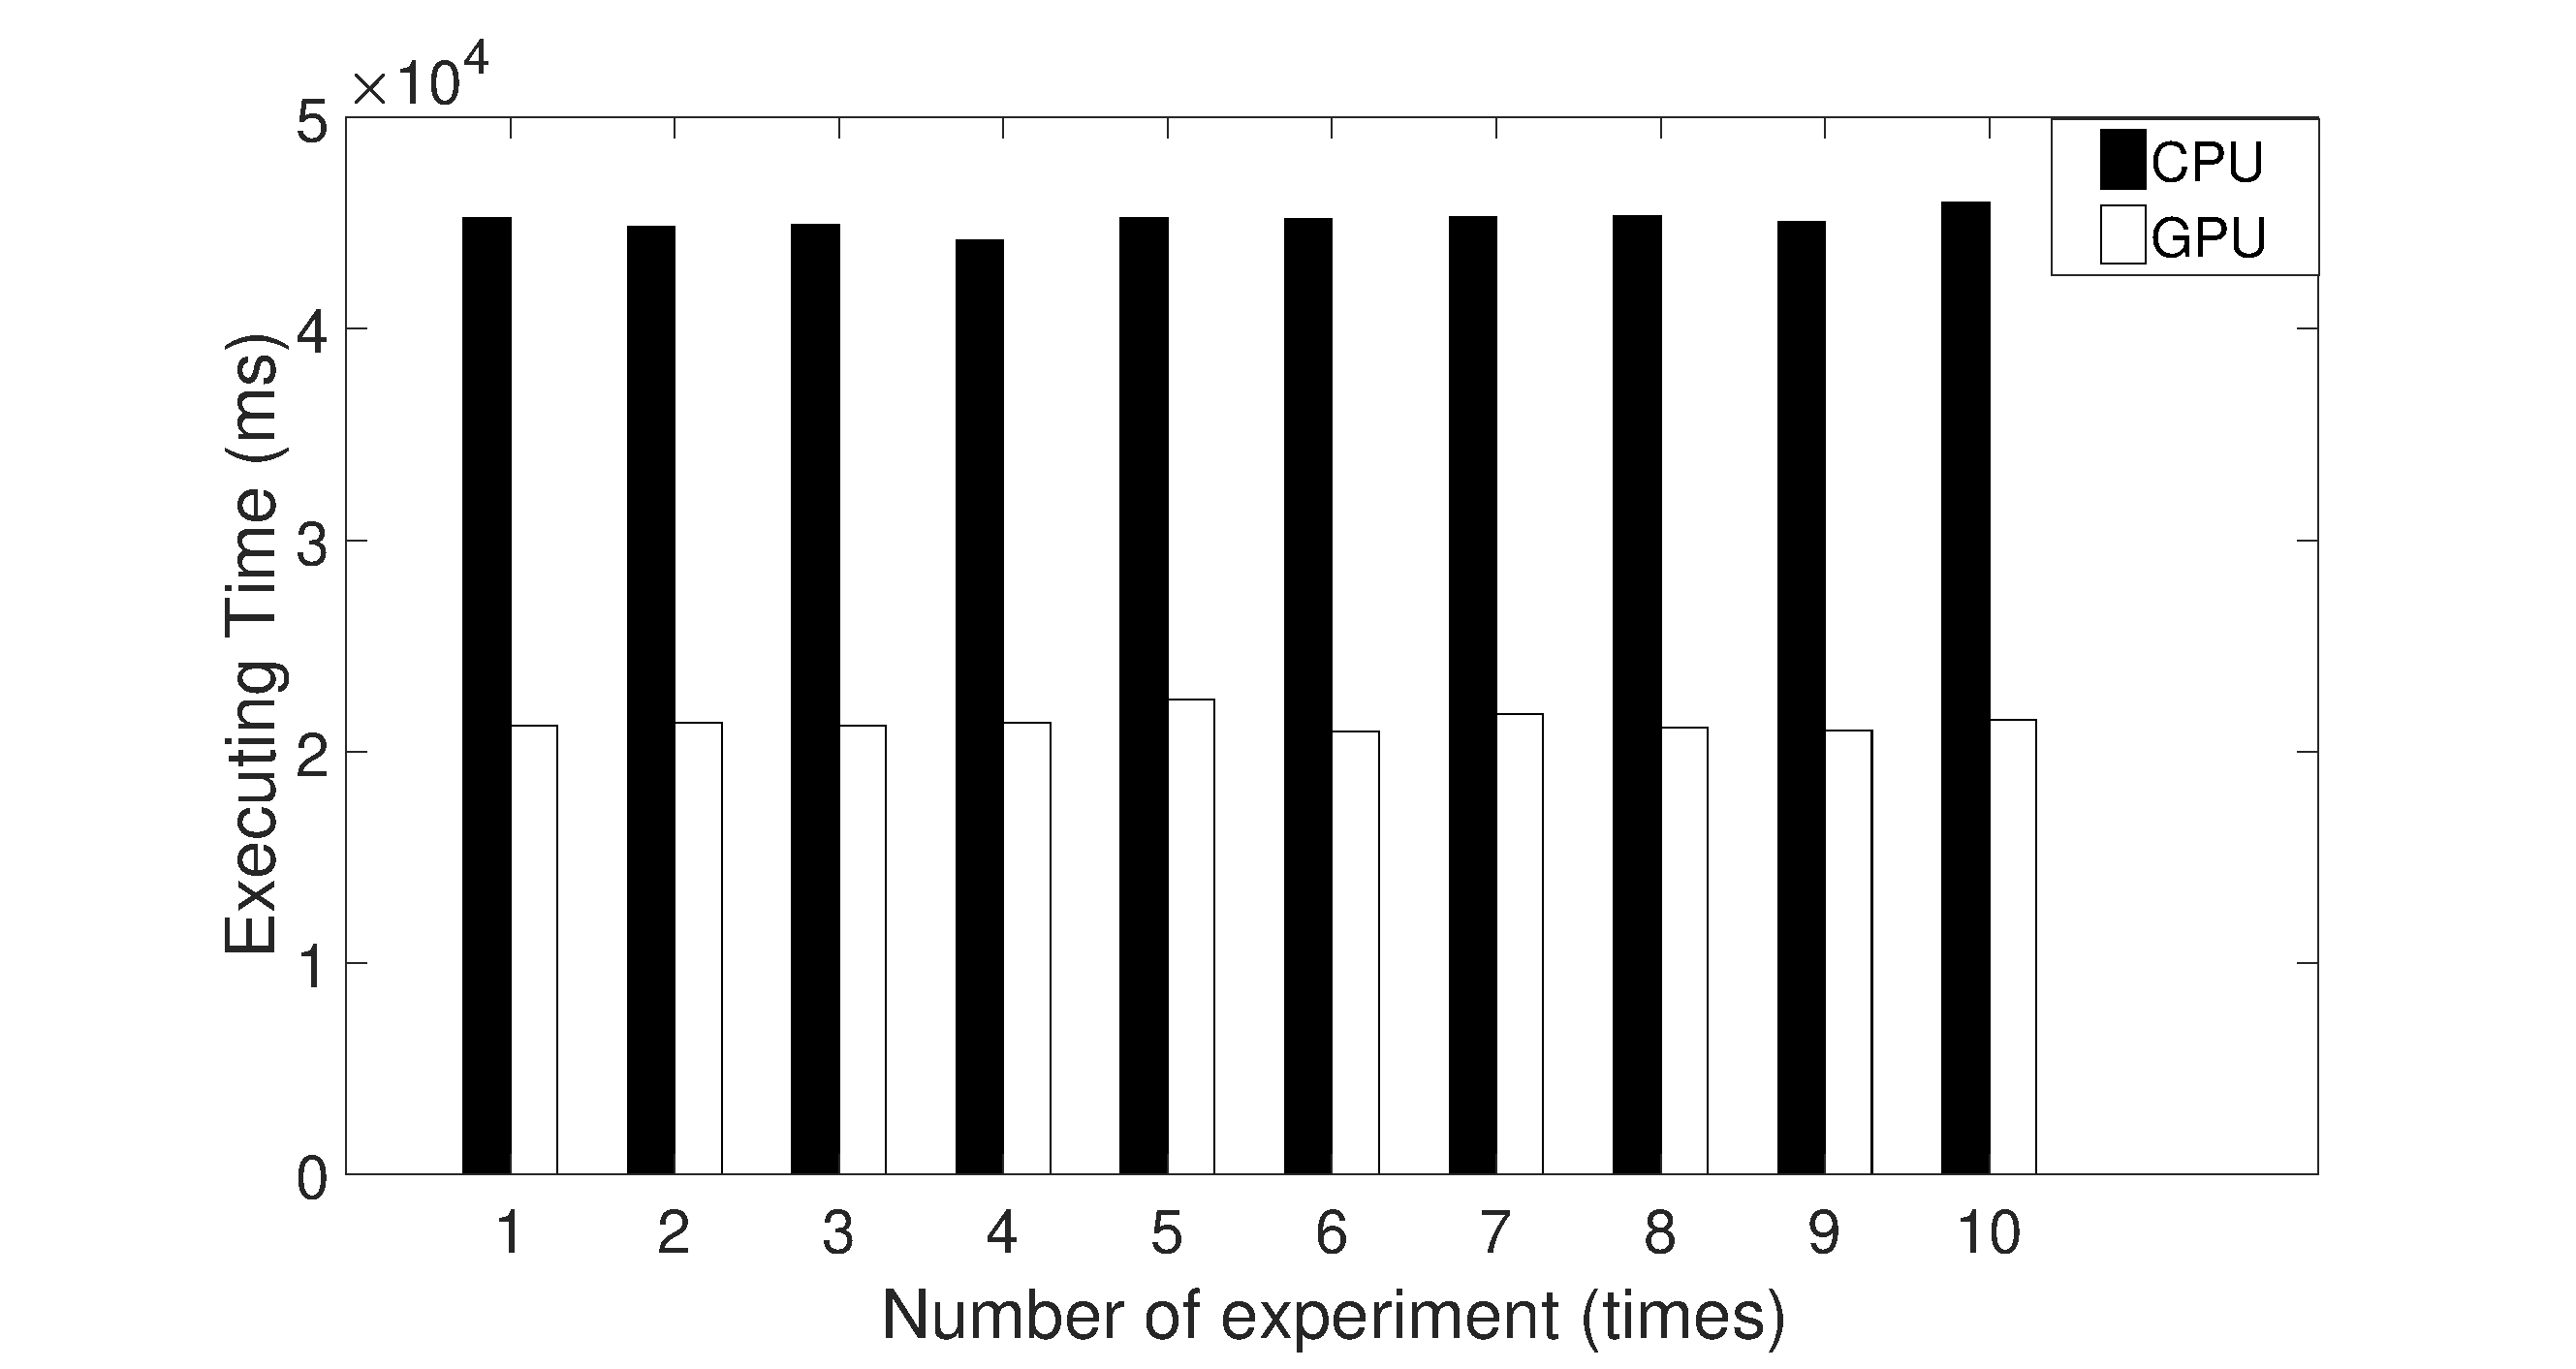
\includegraphics[width=0.8\textwidth]{figures/fig_co2.eps} }
%%   \subfigure[\projectC{}'s Executing Time on CPU is \emph{2.00} times than that on GPU]{
%%     \label{fig:co:c}
%%     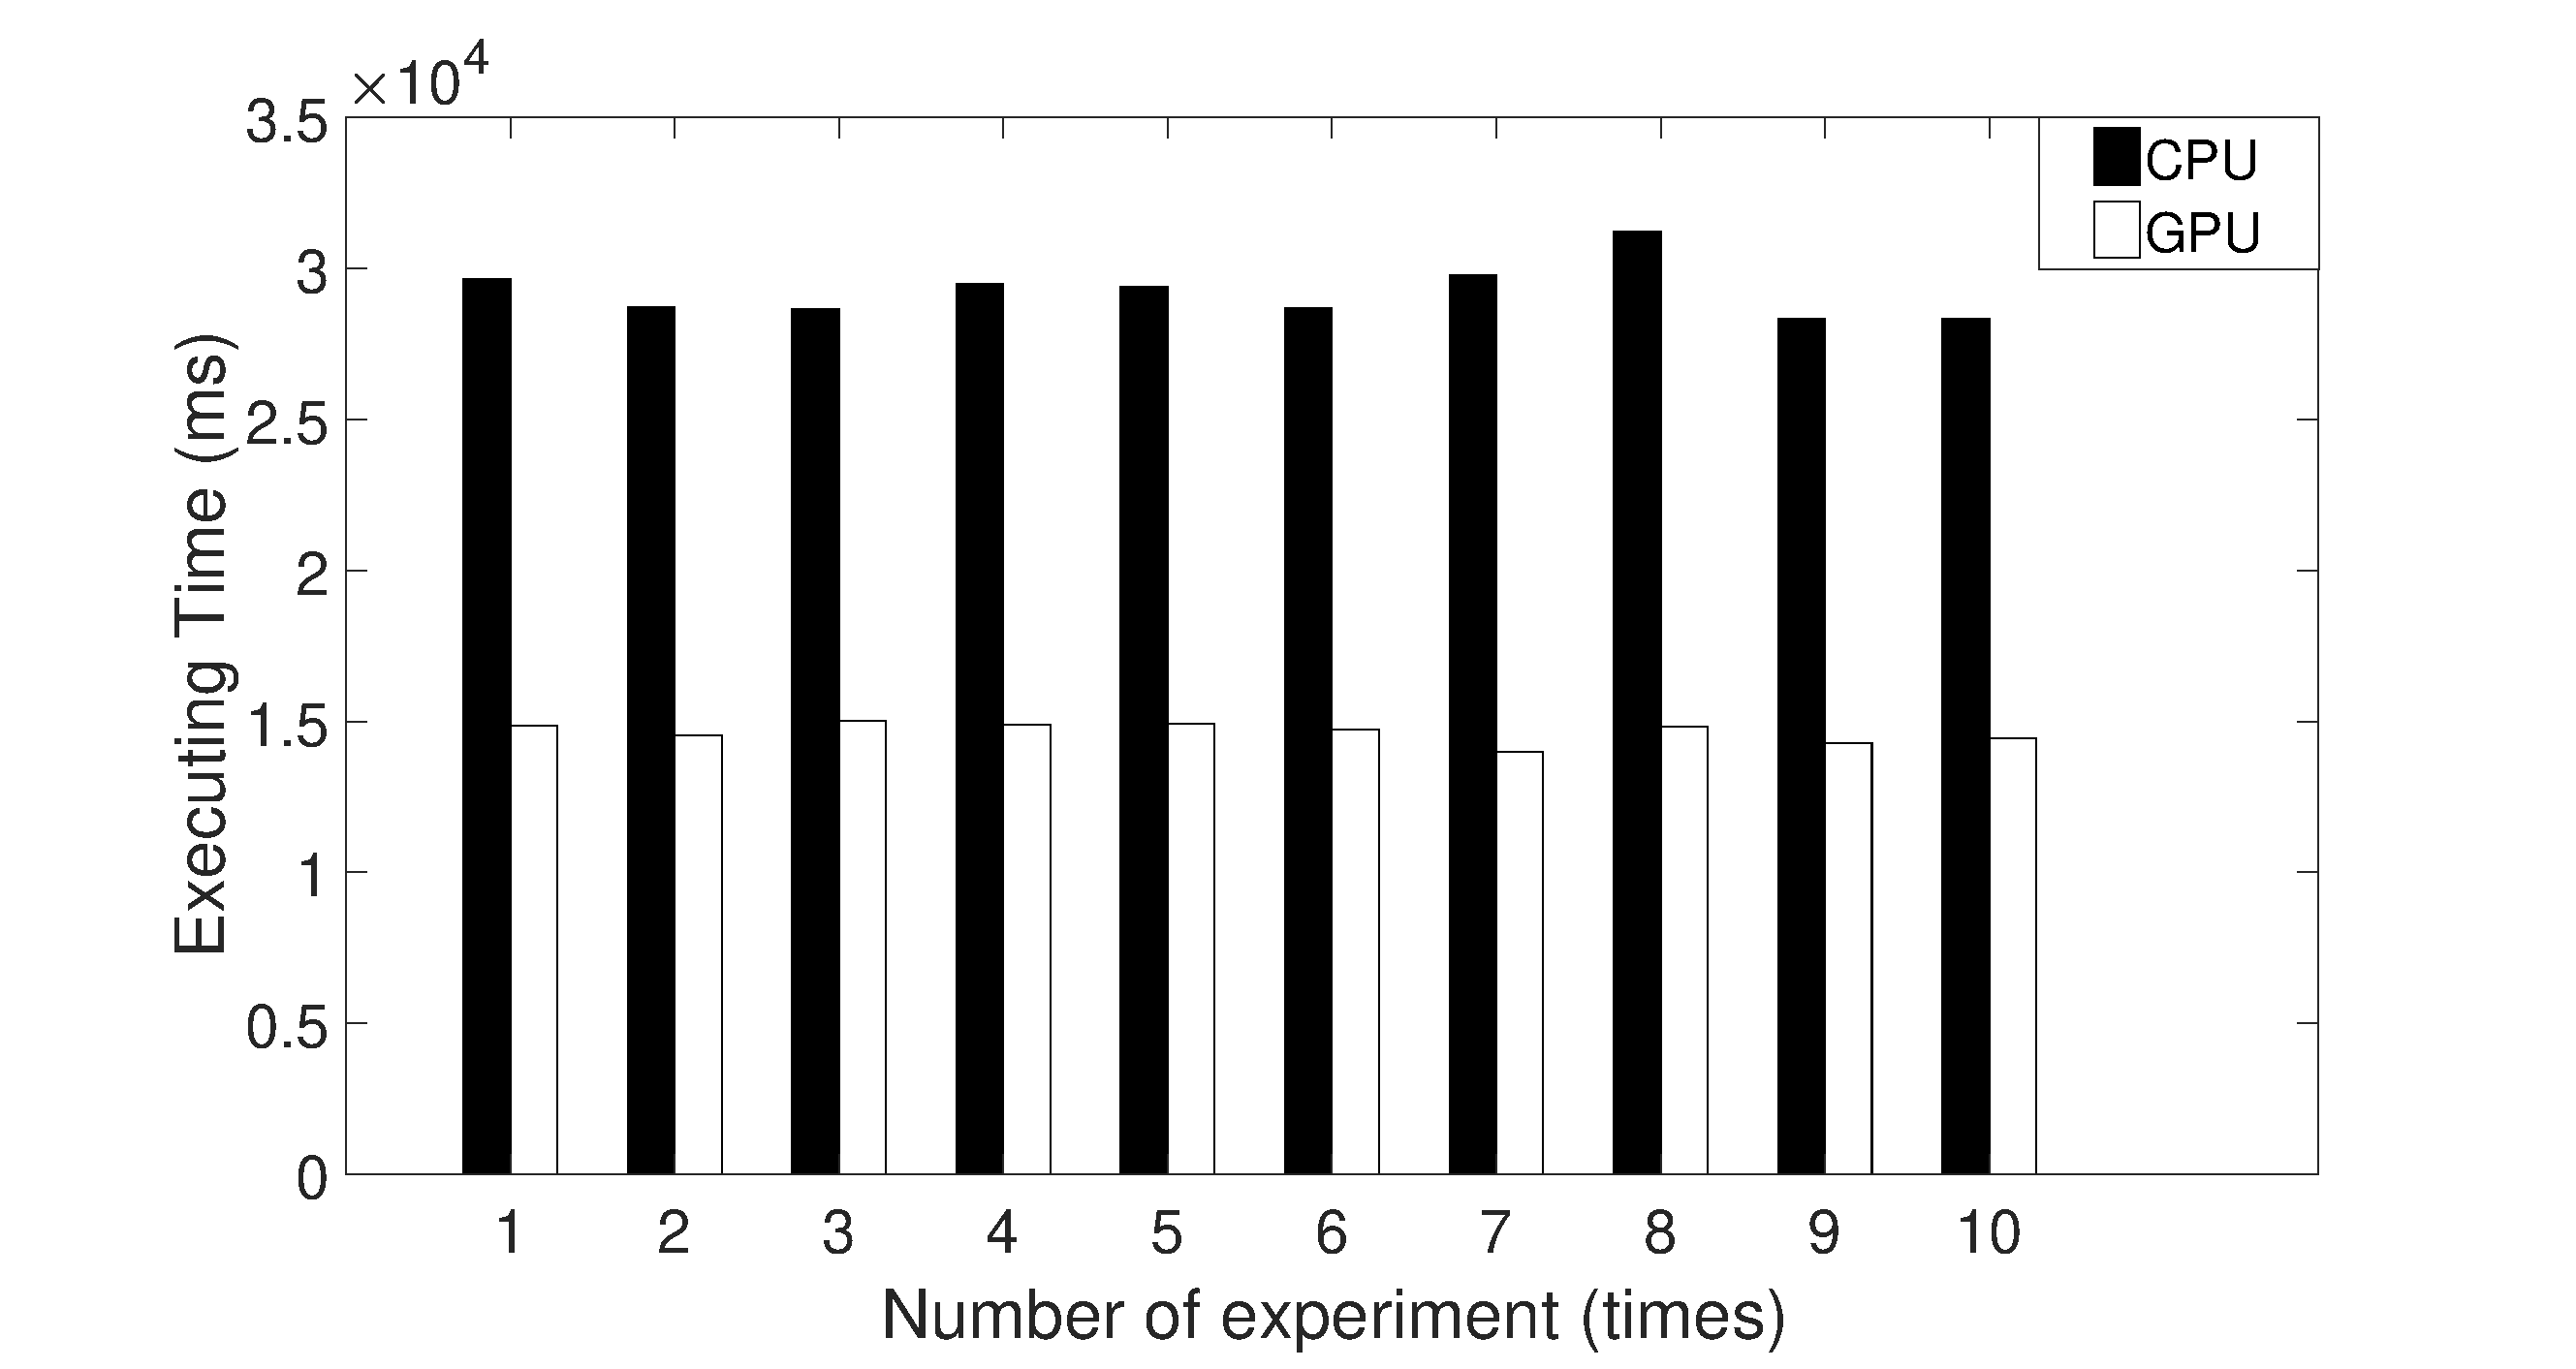
\includegraphics[width=0.8\textwidth]{figures/fig_co3.eps}
%%   }
%%   \caption{Executing Time Comparison of \emph{CPU} and \emph{GPU} Implementation}
%%   \label{fig:co}
%% \end{figure}




% !TEX root = ../paper.tex
%% chapter 6
%\vspace{-6mm}

%\vspace{-3mm}
\section{Related Works}
\vspace{-2mm}

In 1993, Chang et al.~\cite{chang} first proposed the project management problem. The view of
Chang is that software project management net(SPM-Net) can be used to
schedule tasks and manage the resources of software development.
In his article, Chang's project management problem is based on the simulative
data, the reason leading to this is the real industrial data of software
project management is very scanty. In 2007, Alba and Chicano~\cite{alba} optimized the
search algorithms for project management, and solve the project management
problem using genetic algorithm. Their goal is using a search-based approach
to reduce the final completion duration of a project. In 2009, Ren et al.~\cite{ren} first
applied co-evolutionary algorithms to solve project management problem.
Recently, Sarro et al.~\cite{sarro} proposed a a multi-objective decision support approach to help
balance project risks and duration against overtime, so that software
engineers can better plan overtime.
At present, the search space of the work package based on the project
management is more and more huge, the sequential algorithm is not so
effective to solve such problems. Thus, finding a parallel algorithm has
become a hot topic on research~\cite{pentico}.


In recent years, search-based project management problem has become an
important branch of search-based software engineering, and has become a new
field of research. At the same time, the number of papers related to search-
based project management problem is also rising, which makes many researchers
willing to engage in search-based project management problem, so in turn
provides a new platform for practice and innovation of the search-based
project management problem~\cite{penta}.
In 2011, Thomas~\cite{thomas} proposed an approach to describe software project problems
with a set of multiobjective criteria for portfolio managers using the COCOMO II model and
introduce a multiobjective evolutionary approach.
In 2014, Samanta~\cite{samanta} gone through a very brief idea on Genetic Algorithm and implemented the algorithm using MATLAB.
The search-based algorithm is a compute-intensive method, which means the
computer's CPU will be used usually consumed a lot. Therefore, the traditional
sequential computing model cannot meet the requirement of increasing calculation
speed. In 2007, Alba and Chicano~\cite{pospichal} began using search-based methods to improve the
optimal solution of problems, and for the first time using a parallel code model to test the efficiency of search-based methods.
In 2012, Jing~\cite{jing} began solving software project scheduling problems with ant colony optimization.
In recent years, more search-based software engineering methods (such as simulated
annealing, climbing algorithms, evolutionary algorithms, tabu search, etc.) have
been used to solve project management problem, and these methods are usually
able to get good convergence solution on project management problem.

As the development of the algorithm, how to speed up the calculation of the algorithm
has become a hot spot in academic community.
In 2012, Zhang et al.~\cite{zhang} apply GPGPU to
simulation for complex scenes and later on they proposed a GPU-based parallel MOEAs~\cite{li}.
CUDA is a generic parallel computing architecture developed by NVIDIA, which can be used to improve the performance of GPGPU~\cite{langdon2} and also can be optimized by meta-heuristic algorithms~\cite{langdon1,langdon3}.
In 2014, Jianmei~\cite{jianmei} proposed five novel parallel algorithms for solving 
Multi-Objective Combinatorial Optimization problems exactly and efficient.
In general, the parallel evolution algorithm can be implemented on the GPU platform using the CUDA~\cite{vidal}. With the development of the technology of parallelism, a general-purpose GPU(GPGPU) is used
to improve the speed of calculation in software engineering. 


%\textbf{THIS PARAGRAPH TALK TO TOOL, TO BE DELETED???}
In general, a common project management tool which deal with
the mathematical models have not been implemented, so it is difficult to apply
the theory to the industrial project management process. In 2012, Stylianou~\cite{stylianou} and
Gerasimou first developed a tool for project management, which they named
IntelliSPM. The tool uses Matlab and Java programming language and
supports staffing arrangement and resource allocation optimization. In
their work, Stylianou uses the fitness function to dynamic calculate the
dependencies between work packages, so the real project's dependencies may be
broken during the calculation. So in current software engineering practice, the
tool supporting project management is still lacking.


% !TEX root = ../paper.tex
%
% ---------- chapter 7 ----------
%
%\vspace{-3mm}

\section{Conclusions and Future Work}
\vspace{-2mm}

This paper introduces a framework to solve the work package scheduling problem as a single objective optimization problem. The framework accelerates the optimization process by parallelizing the evolving of solutions on a graphic card. 
We conducted a ``proof of concept'' empirical study using data from three industrial software projects, aimed at demonstrate the effectiveness and efficiency of proposed framework.
Results show that the population converge around 20 generations and the parallel version of single objective evolutionary algorithm spend half of the execution time compared to the sequential version, even with only one relative cheap hardware. 
Therefore, we claim that heuristics provides manager with intuitive features towards ``simple-to-deploy'', and parallel computation running on GPU provides shorter execution time.

Future work aims at extending the study reported in this paper with further data sets and accelerating hardware with more cores, above all, at considering a more sophisticated project model, which accounts for further factors not considered in this study, such as group configuration of staff and the interaction among staffing and scheduling.  Future work will also include developing a set of automation tools and techniques. We believe that a optimization tool can automatically parsing a Microsoft Project file (.mpp) can be made useful to provide optimized solutions to aid the managers in practice.
\vspace{-4mm}
\subsubsection{\small{Acknowledgements:}} \small{This work was supported by the State Key Laboratory of Software Development Environment (SKLSDE-2017ZX-20) and the National Natural Science Foundation of China (61602021).}
\vspace{-3mm}

% SKLSDE-2017ZX-20
% 61602021

%
% ---- Bibliography ----
%
\begin{thebibliography}{}
%
\bibitem[1]{stellman}
A. Stellman, and J. Greene.:
Applied Software Project Management.
OREILLY, (2005)

\bibitem[2]{chang}
C. K. Chang, H. Jiang, Y. Di, D. Zhu, and Y. Ge.:
Time-line Based Model for Software Project 
Scheduling with Genetic Algorithms.
Information and Software Technology, 1142-1154 (2008)

\bibitem[3]{alba}
E. Alba, and C. J. Francisco.:
Software Project Management with GA.
Information Sciences, 2380-2401 (2007)

\bibitem[4]{ren}
J. Ren, M. Harman, and M. D. Penta.:
Cooperative Co-evolutionary Optimization of Software 
Project Staff Assignments and Job Scheduling.
Lecture Notes in Computer Science, Springer Berlin Heidelberg, 495-519 (2011)

\bibitem[5]{pentico}
D. W. Pentico.:
Assignment Problems: A Golden Anniversary Survey.
European Journal of Operational Research, 774-793 (2007)

\bibitem[6]{penta}
M. D. Penta, M. Harman, and G. Antoniol.:
The Use of Search-based Optimization Techniques to 
Schedule and Staff Software Projects: An Approach and an Empirical Study. 
Software: Practice and Experience, 495-519 (2011)

\bibitem[7]{pospichal}
P. Pospichal, J. Jaros, and J.:
Schwarz. Parallel Genetic Algorithm on the CUDA Architecture.
Lecture Notes Computation Science, 442-451 (2010)

% \bibitem[8]{qu}
% 曲婉玲, 刘田.:
% 算法设计与分析.
% 北京:清华大学出版社, 205-207 (2011)

\bibitem[9]{stylianou}
C. Stylianou, S. Gerasimou, and A. S. Andreou.:
A Novel Prototype Tool for Intelligent Software 
Project Scheduling and Staffing Enhanced with Personality Factors.
IEEE 24th International Conference on Tools with Artificial Intelligence. 277-284 (2012)

\bibitem[10]{samanta}
S. Samanta.:
Genetic Algorithm: An Approach for Optimization (Using MATLAB). 
International Journal of Latest Trends in Engineering and Technology, 261-267 (2014)

\bibitem[11]{holland}
J. H. Holland.:
Adaptation in Natural and Artificial Systems: an Introductory 
Analysis with Applications to Biology, Control, and Artificial Intelligence.
U Michigan Press, (1975)

\bibitem[12]{harman}
M. Harman, P. McMinn, J. T. D. Souza, and S. Yoo.:
Search Based Software Engineering: Techniques, Taxonomy, Tutorial.
Empirical software engineering and verification, 1-59 (2012)

\bibitem[13]{deb}
K. Deb, A. Pratap, S. Agarwal, and T. Meyarivan.:
A Fast and Elitist Multiobjective Genetic Algorithm: NSGA-II.
IEEE Transactions on Evolutionary Computation, 182-197 (2002)

\bibitem[14]{vidal}
P. Vidal, and E. Alba.:
A Multi-GPU Implementation of a Cellular Genetic Algorithm.
2010 IEEE World Congress on Computational Intelligence, 1-7 (2010)

% \bibitem[15]{kirk}
% D.B. Kirk, W. W. Hwu.:
% 大规模并行处理器编程实战(第二版).
% 北京: 清华大学出版社, 1-31 (2013)




% ---------------------------------
% \bibitem[1980]{2clar:eke}
% Clarke, F., Ekeland, I.:
% Nonlinear oscillations and
% boundary-value problems for Hamiltonian systems.
% Arch. Rat. Mech. Anal. 78, 315--333 (1982)

% \bibitem[1981]{2clar:eke:2}
% Clarke, F., Ekeland, I.:
% Solutions p\'{e}riodiques, du
% p\'{e}riode donn\'{e}e, des \'{e}quations hamiltoniennes.
% Note CRAS Paris 287, 1013--1015 (1978)

% \bibitem[1982]{2mich:tar}
% Michalek, R., Tarantello, G.:
% Subharmonic solutions with prescribed minimal
% period for nonautonomous Hamiltonian systems.
% J. Diff. Eq. 72, 28--55 (1988)

% \bibitem[1983]{2tar}
% Tarantello, G.:
% Subharmonic solutions for Hamiltonian
% systems via a $\bbbz_{p}$ pseudoindex theory.
% Annali di Matematica Pura (to appear)

% \bibitem[1985]{2rab}
% Rabinowitz, P.:
% On subharmonic solutions of a Hamiltonian system.
% Comm. Pure Appl. Math. 33, 609--633 (1980)

\end{thebibliography}
\clearpage

% end of bibliography


\end{document}
